\documentclass[12pt]{article}
%\usepackage{nopageno}
\usepackage{subfiles}
\usepackage{graphicx}
\usepackage[margin=1in]{geometry} 
\usepackage[UKenglish]{isodate}
\usepackage{amsmath,amsthm,amssymb}
\usepackage{longtable}
%\usepackage{enumerate}
\usepackage[shortlabels]{enumitem}
\setlistdepth{9}
\newlist{longenum}{enumerate}{6}
\setlist[longenum,1]{label=\arabic*.}
\setlist[longenum,2]{label=\alph*.}
\setlist[longenum,3]{label=\roman*.}
\setlist[longenum,4]{label=\arabic*.}
\setlist[longenum,5]{label=\alph*.}
\setlist[longenum,6]{label=\roman*.}
%\setlist[longenum,7]{label=\arabic*.}
\usepackage[separate-uncertainty=true]{siunitx}
\sisetup{range-phrase=--}
\usepackage{mhchem}
\usepackage{hyperref}
\usepackage{mathpazo}
%\usepackage[dvipsnames]{xcolor}
\usepackage{comment}
%\usepackage{multirow}
\usepackage{tikz}
\usetikzlibrary{positioning,calc}
\usepackage{pgfplots}

\usepackage{fancyhdr}
\pagestyle{fancy}
%\fancyfoot[LE,RO]{\thepage}

\setcounter{section}{-1}

\title{The Great Big Astro Lab Manual}
\author{Yvonne Ban}
%\date{}
\cleanlookdateon

\begin{document}
\begin{titlepage}

\maketitle
\begin{center}
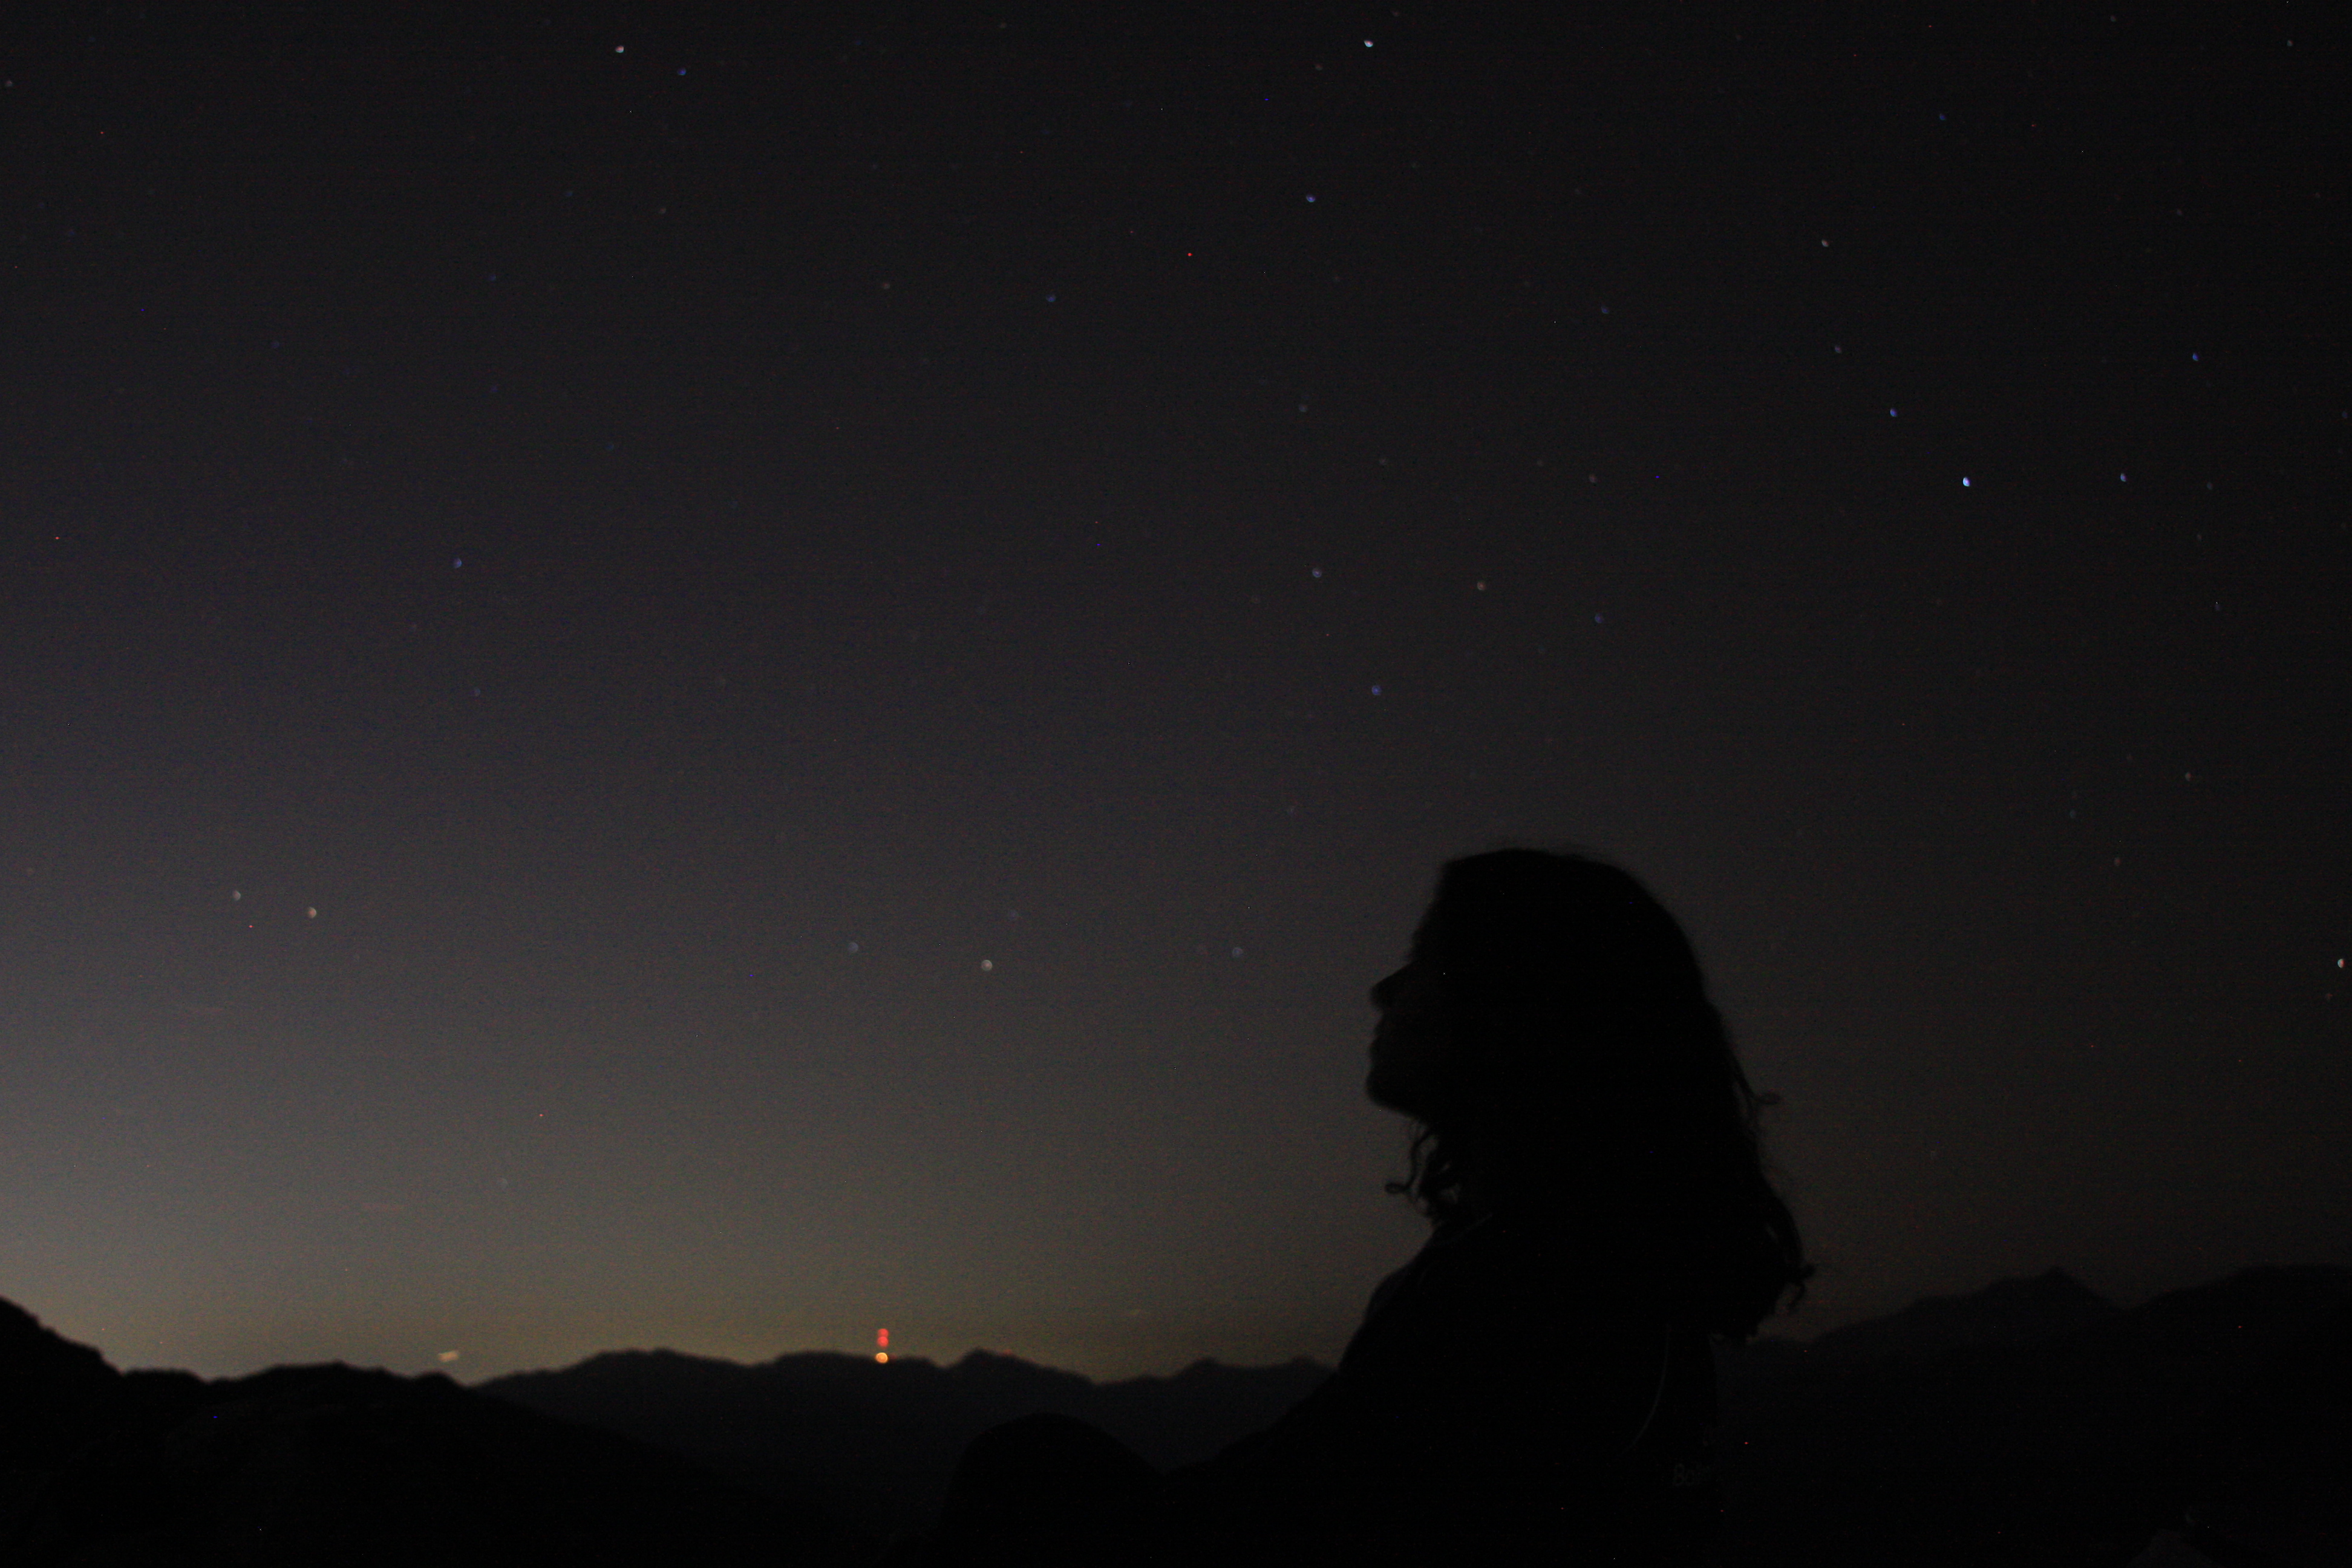
\includegraphics[width=\textwidth]{IMG_0499.JPG}
Cow Canyon Saddle, Mt. Baldy, Los Angeles, CA, USA. Yvonne Ban, 24 Oct 2014. Model: Emily Schooley
\end{center}

\thispagestyle{empty}
\clearpage
\pagenumbering{arabic}

\end{titlepage}
%\newpage

\tableofcontents

\section*{Preface}
\addcontentsline{toc}{section}{Preface}


\section{How to use this manual}

Hello friend! Welcome to my masterwork.


\subsection{Manual}


\subsection{Worksheets and Handouts}


\subsection{Using tex files}


\section{Introduction}

Astronomy is the study of the heavens. As such, a fundamental limitation of the subject is that we do not, in general, conduct \emph{experiments}, only \emph{observations} where we snatch jealously at the sparing scraps of information tantalisingly offered by nature. One could argue that astronomy lives at the very cutting edge of our knowledge, where the scientific exercises of hypothesis formulation and testing are most active and challenging.

Such lofty heights of intellectual endeavour are difficult to convey to the next generation of scientists; astronomy draws on physics, chemistry, mathematics, engineering, programming and computer science at an ever increasing rate, and sometimes even biology. Overwhelmingly, astronomy in the academic institution is presented either in lectures or in research projects involving data from observations. The lucky few may even get the opportunity to personally participate in a physical observation run at one of the awe-inspiring cathedrals of science that are the observatories. None of these formats apply to the Astronomy Lab.

Instead, Astronomy Lab is not so much about \emph{experiments} but more about the \emph{models} that we use in astronomy, which play a larger part in the formation of knowledge in astronomy as compared to other subjects. The in-class activities of the course provide an opportunity to teach students about astronomical models in a more engaged and hands-on manner than can be accomplished in a lecture. Using a variety of excellent pedagogical materials, ranging from web apps and planetarium software to experiments and physical models that the students construct themselves, the goal of the course is to use kinesthetic and self-guided exploration to let students learn and internalise the concepts and models of astronomy.

This manual was precipitated by the COVID-19 pandemic, which caused schools to transition to remote learning. Through adapting this course for this mode, sometimes being as remote as the other side of the Earth, and then adapting it back to in-person classes, we drew from the trials and experiences therewith to formalise a robust programme that will minimise the work needed to plan and oversee the conduction of the course.

\section{Setup}

\subsection{Course setup}

The Astronomy 100/1 Lab is conducted in tandem with the Astronomy 100 and(/or) 101 courses and is required to be taken simultaneously.


\subsubsection{Schedule}

Each semester, 6 independent sections are held on Monday, Wednesday, and Friday of every school week at 12:20-1:10pm (1220-1310) and 1:25-2:15pm (1325-1415). Generally, a lead teaching assistant (TA) and assistant TA is assigned for each section. The workload can be split up amongst the assigned TAs so that each section is covered. There may also be assistance from undergrad TAs.


\subsubsection{Scripting}

I have designed it such that most of the script for each class can be essentially read off the slides. You can also reference the teaching notes for more details.


\subsubsection{Technical details}

Every class is held in the Integrated Learning Center (ILC) room S220. The room consists of:
\begin{itemize}
\item 11 round tables at which students sit with power points (and table microphones)
\item 3 physically secured Macbooks at each table that can be accessed with one’s NetID and have Stellarium installed
\item 1 central instructor’s (standing) desk (“lectern") with elevated chair
\item 1 lectern computer controlling lights and A/V of room
\item Lights with 3(?) brightness settings
\item 2 wireless microphones, one handheld, one wired clip-on
\item 2 HDMI and VGA feeds each, “Lectern Laptop" and “Lectern Aux"
\item Digital document projector on left side of instructor’s desk, “Document Cam"
\item Whiteboards that wrap around the room
\item 11 eye-level screens with 2 separate feeds, “A" and “B", one located nearest each table
\item 4 screens located above instructor’s desk, “Stadium"
\end{itemize}


\subsection{Materials}

Every student gets an individual lab worksheet for each lab. Activities that involve teamwork at each table may have a table worksheet for each table. Copies of the syllabus and Stellarium guide may also be provided in hard copy. All materials and instructor presentations are copied on the class webpage on Moodle (Moonami, or Moodle in the Cloud).

All individual student submissions, including all end-of-class quizzes, are administered on Moodle. Table teams fill out and submit table worksheets in class.

Demo materials for specific labs are listed for each lab and can be found in the class supply room.


\subsection{Grade breakdown}

The total Astronomy Lab grade makes up 25\% of the overall Astronomy 100/1 course grade, and does not have a separate grade. The remaining 75\% of the Astronomy 100/1 course grade comes from lecture assignments and exams. Within Astronomy Lab, the grade assignment is broken down as shown in Table ~\ref{tab:grades}.

\begin{table}[htbp]
\centering
\caption{Breakdown of grade assignments for Astronomy 100/1 Lab}
\begin{tabular}{|l|l|l|}\hline
Lab & Component & \% \\\hline
1 & Background knowledge survey & 7 \\ 
& Quiz & 3 \\\cline{2-3}
& Total & 10 \\\hline
2 & Quiz & 10 \\\cline{2-3}
& Total & 10 \\\hline
3 & Survey & 2 \\ 
& Quiz & 8 \\\cline{2-3}
& Total & 10 \\\hline
4 & Survey & 2 \\ 
& Quiz & 8 \\\cline{2-3}
& Total & 10 \\\hline
5 & Survey & 2 \\ 
& Quiz & 8 \\\cline{2-3}
& Total & 10 \\\hline
6 & Survey & 2 \\ 
& Quiz & 8 \\\cline{2-3}
& Total & 10 \\\hline
7 & Survey & 2 \\ 
& Quiz & 8 \\\cline{2-3}
& Total & 10 \\\hline
8 & Survey & 2 \\ 
& Quiz & 8 \\\cline{2-3}
& Total & 10 \\\hline
Sunset photo project & Photo policy & 1 \\ 
& Calibration photos & 2 \\
& 1st sunset photo and location & 9+1 \\
& 2nd sunset photos & 8+1 \\\cline{2-3}
& Total & 20+2 \\\hline
Extra credit project & Photos & 5 \\ 
& Report & 5 \\\cline{2-3}
& Total & 10 \\\hline
\end{tabular}
\label{tab:grades}
\end{table}


%\newpage
\subsubsection{Manual grading rubrics}

Sunset(/sunrise) photo project (20+2)
\begin{longenum}
\item 1st photo (10+1)
    \begin{longenum}
    \item Auto (3)
        \begin{longenum}
        \item Photo policy (1)
        \item Calibration photos (2)
        \end{longenum}
    \item Manual (7+1)
        \begin{longenum}
        \item Photos (7)
        	\begin{longenum}
            \item 1st sunset photo (5)
                \begin{longenum}
                \item Photo exists and correct format (1)
                \item Sun location (3)
                    \begin{longenum}
                    \item Azimuth discernible (1)
                        \begin{itemize}
                        \item -1 Sun's position along the horizon is unclear
                        \end{itemize}
                    \item Altitude discernible (1)
                        \begin{itemize}
                        \item -1 Sun's position is unclear
                        \end{itemize}
                    \item Altitude within 5 to -1 deg above horizon (1)
                        \begin{itemize}
                        \item -1 Sun is too far above the horizon
                        \item -1 Sun is below the horizon
                        \end{itemize}
                    \end{longenum}
               \item Horizon (1)
                    \begin{longenum}
                    \item Visible (0.5)
                        \begin{itemize}
                        \item -0.5 Horizon is not visible
                        \end{itemize}
                    \item Features (0.5)
                        \begin{itemize}
                        \item -0.5 Horizon has no features
                        \end{itemize}
                    \end{longenum}
                \end{longenum}
            \item Location photo (2)
                \begin{longenum}
                \item Location discernible (1)
                    \begin{itemize}
                    \item -1 Location unclear
                    \end{itemize}
                \item Location repeatable (1) 
                    \begin{itemize}
                    \item -1 Location not accurately enough indicated
                    \end{itemize}
                \end{longenum}
            \end{longenum}
        \item Early (on-time) submission (+1)
        \end{longenum}
    \end{longenum}
\item 2nd and 3rd photos (8+1)
    \begin{longenum}
    \item Auto (2)
    \item Manual (6+1)
        \begin{longenum}
        \item Photos (2+1)
            \begin{longenum}
           \item 2nd photo (2)
                \begin{longenum}
               \item From exact same spot (0.5)
                    \begin{itemize}
                    \item -0.5 Location changed
                    \end{itemize}
                \item Date is $\geq$ 1 week after 1st sunset (0.5)
                    \begin{itemize}
                    \item -0.5 Too close to 1st photo
                    \end{itemize}
                \item Sun can be located (0.5)
                    \begin{itemize}
                    \item -0.5 Sun cannot be located
                    \end{itemize}
                \item Horizon visible + Sun close enough to horizon (0.5)
                    \begin{itemize}
                    \item -0.5 Horizon cannot be seen or too far from sunset
                    \end{itemize}
                \end{longenum}
            \item 3rd photo (+1)
                \begin{longenum}
                \item Attempt (0.5)
                \item Successful (0.5)
                \end{longenum}
            \end{longenum}
        \end{longenum}
        \item Quiz (4)
            \begin{longenum}
            \item Short essay (1)
                \begin{longenum}
                \item Agrees with annotated picture (0.5)
                    \begin{itemize}
                    \item Sunset locations
                    \item Picture scale
                    \end{itemize}
                \item Sensible (0.5)
                \end{longenum}
            \end{longenum}
            \item Annotated picture (3)
                \begin{longenum}
                \item $\geq 3$ Locations marked (1)
                    \begin{itemize}
                    \item -0.5 Location missing
                    \item 2 locations missing means 0
                    \end{itemize}
                \item Annotations (1)
                \item Locations reasonable (1)
                    \begin{longenum}
                    \item Summer (winter) solstice sunset(/-rise) is East (West) of earlier sunsets(/-rises) (0.5)
                        \begin{itemize}
                        \item -0.5 Summer (winter) solstice sunset(/-rise) location wrong 
                        \end{itemize}
                    \item To scale (0.5)
                        \begin{itemize}
                        \item -0.5 Locations not marked to scale
                        \end{itemize}
                    \end{longenum}
                \end{longenum}
    \end{longenum}
\item End-of-lab quiz (2)
    \begin{longenum}
    \item Auto (2)
    \end{longenum}
\end{longenum}

Extra credit Moon photo project (10)
\begin{longenum}
\item Auto (1)
    \begin{longenum}
    \item Quiz question (1)
    \end{longenum}
\item Manual (9)
    \begin{longenum}
    \item Photos (5)
        \begin{longenum}
        \item Uploaded pictures in readable format (1)
        \item Zoomed-out daytime picture of Moon with horizon visible (2)
            \begin{longenum}
            \item Horizon can be behind something as long as they make clear what's level to camera and use that to estimate Moon's altitude
                \begin{itemize}
                \item -2 Picture not taken in daytime
                \item -1 Picture taken just after sunset
                \end{itemize}
            \end{longenum}
        \item Zoomed-in picture of Moon taken with same camera at same time (1)
        \item Stellarium screenshot makes sense and lists moon parameters (1)
            \begin{itemize}
            \item N.B.: Auto question also asks for Moon parameters 
            \end{itemize}
        \end{longenum}
    \item Essay (4)
        \begin{longenum}
        \item Clear explanation of Moon's altitude relative to the calibration picture (1)
            \begin{itemize}
            \item values don't have to be correct, but see if they compare numerically
            \end{itemize}
        \item Reasonable explanation for how they found size of Moon based on calibration photo (1)
        \item Reasonable explanation of comparison to golf ball (1)
        \item Attached photo of golf ball (1)
        \end{longenum}
    \end{longenum}
\end{longenum}


\newpage
\section{Labs}

%\subsection{Lab 0: this only exists to please my ocd ass}

\subsection{Lab 1: Astronomical Angles and Stellarium}

\subsubsection{Overview}

Topics covered:
\begin{itemize}
\item Angular measurements
\item Using Stellarium
\item Azimuths and Altitudes of astronomical objects
\end{itemize}

\noindent
Watch out for:
\begin{itemize}
\item 
\end{itemize}

\subsubsection{Materials needed}

Instructors:
\begin{itemize}
\item Lab worksheets
\item Syllabus
\item Stellarium guide
\end{itemize}

\noindent
Students:
\begin{itemize}
\item Computer
\end{itemize}


\subsubsection{Script}

\newcommand\slidepath[1]{ppt/lab01/Slide#1.jpeg}

\emph{Before the end of class, set the Moodle Lab Quiz access password.}

\begin{longtable}{|m{0.5\textwidth}|m{0.5\textwidth}|}\hline
Pick up copies of lab worksheet, syllabus, and Stellarium guide. & \includegraphics[width=0.5\textwidth]{\slidepath{1}}\\\hline
Log in to Moodle, go to the Astronomy 100/101 Lab page, and fill out the Astronomy Background Survey. (The survey is graded on participation only.) & \includegraphics[width=0.5\textwidth]{\slidepath{3}}\\\hline
Astronomy Lab grade makes up 25\% of the Astronomy 100/101 total grade.

\textbf{Submitting work or pictures that are not your own, or having someone else do it for you, is dishonest and will be dealt with harshly.}

Lab usually improves your overall grade, if you put in the small time and effort commitment needed. & \includegraphics[width=0.5\textwidth]{\slidepath{5}}\\\hline
If you miss a lab, look out for at-home makeups or scheduled makeup labs, and try to let us know ASAP.

Don't procrastinate on the project; it's not difficult, but is impossible if left to the last minute. & \includegraphics[width=0.5\textwidth]{\slidepath{7}}\\\hline
Stellarium is a planetarium software that simulates what the sky looks like at different locations and times. & \includegraphics[width=0.5\textwidth]{\slidepath{8}}\\\hline
If you're using a lab computer, Stellarium is already installed and you can just pull it up. If you're using your own computer, download the correct installer from this website and install it. If your OS isn't available, you can use the web version. Open the Location Window from the left-hand menu panel or by pressing F6. In the search bar under the top right menu, type ``Amherst" and select ``Amherst Center, United States".

Take note that it's ``Amherst Center", not ``Amherst" (that's in NY somewhere). Also, \textbf{do not type} into the ``Name/City" box. That renames the location.

Close the window and open the Date/Time Window from the left-hand menu panel or by pressing F5. Set the time to 7:00pm tonight to see what will be visible.

Practice dragging the view with the cursor to view different directions. Note that to zoom in, you scroll \textbf{up}, and to zoom out, you scroll \textbf{down}. & \includegraphics[width=0.5\textwidth]{\slidepath{9}}\\\hline
In astronomy, we use angles to measure positions and separations of objects in the sky. Your position is measured by latitude and longitude. (These are angles measured with the vertex at the centre of the Earth. Where is the angle of your position measured relative to?) & \includegraphics[width=0.5\textwidth]{\slidepath{10}}\\\hline
From your point of view, an object's position is given by \textbf{azimuth} and \textbf{altitude}. Similar to before, we take the vertex of the angle measurement to be your position. For altitude, the angle is measured relative to the horizon. For azimuth, the angle is measured relative to due north. & \includegraphics[width=0.5\textwidth]{\slidepath{11}}\\\hline
To compare astronomical positions independent of observer location, we use the celestial coordinate system. It's very similar to latitude and longitude, which correcpond to declination and right ascension respectively. & \includegraphics[width=0.5\textwidth]{\slidepath{12}}\\\hline
Astronomers use the \textbf{sexagesimal} system for recording angles. Each degree is divided into 60 \textbf{arc minutes} (\si{\arcminute}), and each arc minute is divided into 60 \textbf{arc seconds} (\si{\arcsecond}).

Right ascension also measures angle, but it is measured like how we measure time, in hours-minutes-seconds. In right ascension, there are 24 hours in a circle of 360 \si{\degree}. & \includegraphics[width=0.5\textwidth]{\slidepath{13}}\\\hline
Fill out your worksheet. & \includegraphics[width=0.5\textwidth]{\slidepath{14}}\\\hline
%\emph{At ~10 min from class end, show Moodle quiz password.} 

%Complete the Lab quiz on Moodle.

Remember to complete the pre-lab survey. & 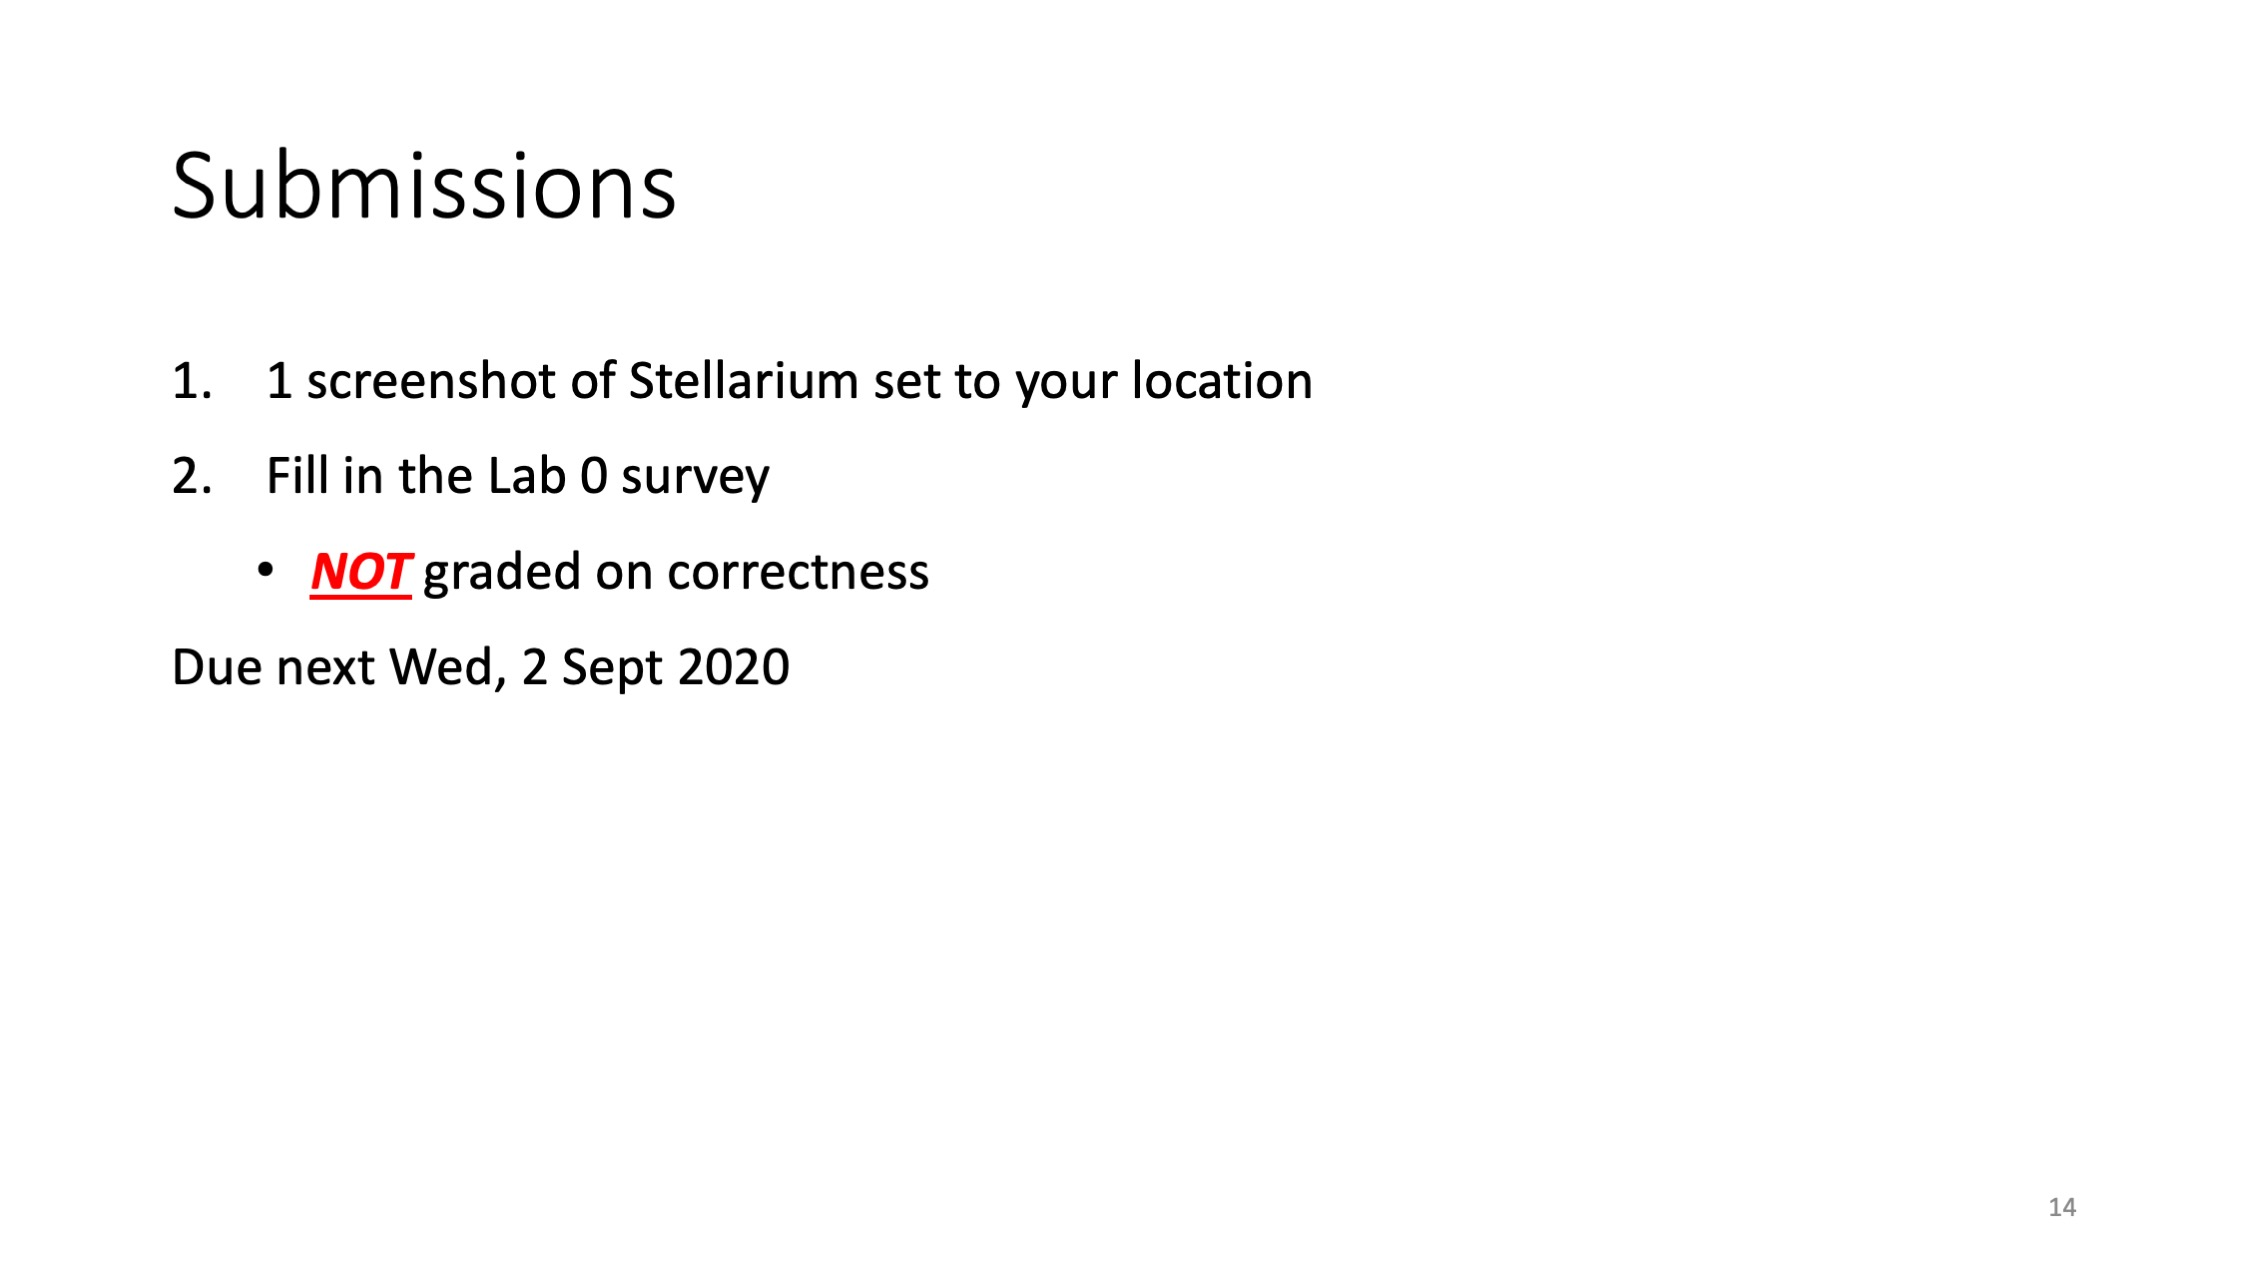
\includegraphics[width=0.5\textwidth]{ppt/lab01/Slide15.jpeg}\\\hline
%\label{default}
\end{longtable}


\subsubsection{Submissions}

Moodle:
\begin{enumerate}
\item Astronomy background survey
\end{enumerate}

\noindent
In-class:
\begin{enumerate}
\item None
\end{enumerate}


\subsubsection{Astronomy Background Survey}

This survey is given before any instruction is given, and questions 1-11 are surveyed again at the end of the course.

\begin{enumerate}
\item
As seen from Amherst, MA, when will an upright flagpole cast no shadow because the Sun is directly above the flagpole?
\begin{itemize}
    \item Everyday at noon.
    \item Only on the first day of summer.
    \item Only on the first day of winter.
    \item On both the first days of spring and fall.
    \item \underline{Never.}
\end{itemize}
\item
When the Moon appears to completely cover the Sun (an eclipse), the Moon must be at which phase?
\begin{itemize}
    \item Full
    \item \underline{New}
    \item First quarter
    \item Last quarter
    \item At no particular phase
\end{itemize}
\item
Imagine that you are building a scale model of the Earth and the Moon. You are going to use a 12-inch basketball to represent the Earth and a 3-inch tennis ball to represent the Moon. To maintain the proper distance scale, about how far from the surface of the basketball should the tennis ball be placed?
\begin{itemize}
    \item 4 inches (1/3 foot)
    \item 6 inches (1/2 foot)
    \item 36 inches (3 feet)
    \item \underline{30 feet}
    \item 300 feet
\end{itemize}
\item
Imagine that the Earth's orbit were changed to be a perfect circle about the Sun so that the distance to the Sun never changed. How would this affect the seasons?
\begin{itemize}
    \item We would no longer experience a difference between the seasons.
    \item We would still experience seasons, but the difference would be much LESS noticeable.
    \item We would still experience seasons, but the difference would be much MORE noticeable.
    \item \underline{We would continue to experience seasons in the same way we do now.} 
\end{itemize}
\item
\begin{figure}[htbp]
    \centering
    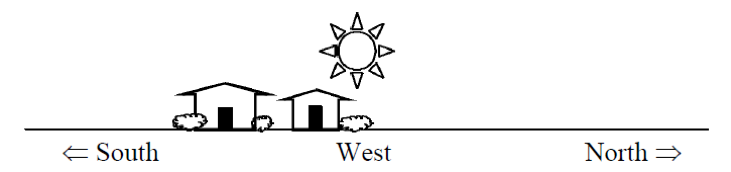
\includegraphics{asq5.png}
    \caption{}
    \label{fig:asq5}
\end{figure}
On about September 22, the Sun sets directly to the west, as shown on the diagram below (Fig.~\ref{fig:asq5}). Where would the Sun appear to set two weeks later?
\begin{itemize}
    \item Farther south
    \item In the same place
    \item \underline{Further north}
\end{itemize}
\item
As viewed from our location, the stars of the Big Dipper can be connected with imaginary lines to form the shape of a pot with a curved handle. What is the closest point you would have to travel to in order to observe a substantial change in the shape formed by these stars?
\begin{itemize}
    \item Across the country
    \item A distant star
    \item Europe
    \item Moon
    \item Pluto
    \item \underline{A distant star}
\end{itemize}
\item%TODO: what's the answer
With your arm held straight, your little fingernail is just wide enough to cover up the Sun. If you were on Saturn, which is 10 times farther from the Sun than the Earth is, which of the following objects could you use to just barely cover up on the Sun?
\begin{itemize}
    \item Your wrist
    \item Your thumb
    \item A pencil
    \item A strand of spaghetti
    \item \underline{A hair}
\end{itemize}
\item
\begin{figure}[htbp]
    \centering
    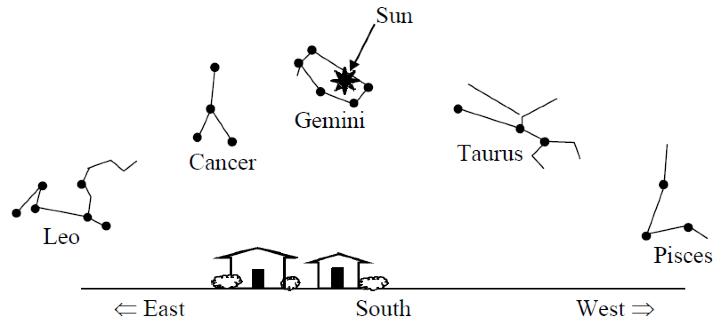
\includegraphics{asq8.png}
    \caption{}
    \label{fig:asq8}
\end{figure}
If you could see stars during the day, this is what the sky would look like at noon on a given day (Fig.~\ref{fig:asq8}). The Sun is near the stars of the constellation Gemini. Near which constellation would you expect the Sun to be located at sunset?
\begin{itemize}
    \item Leo
    \item Cancer
    \item \underline{Gemini}
    \item Taurus
    \item Pisces
\end{itemize}
\item
\begin{figure}[htbp]
    \centering
    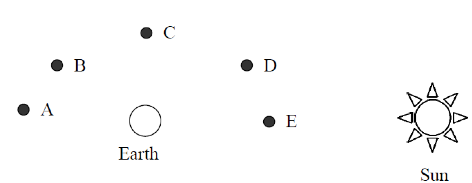
\includegraphics{asq9a.png}
    \caption{}
    \label{fig:asq9a}
\end{figure}
\begin{figure}[htbp]
    \centering
    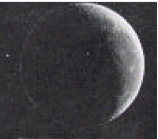
\includegraphics{asq9b.png}
    \caption{}
    \label{fig:asq9b}
\end{figure}
The diagram below (Fig.~\ref{fig:asq9a}) shows the Earth and Sun as well as five different possible positions for the Moon. Which positions of the Moon would cause it to appear like the picture of the Moon below (Fig.~\ref{fig:asq9b}) when viewed from Earth?
\begin{itemize}
    \item A
    \item B
    \item C
    \item \underline{D}
    \item E
\end{itemize}
\item
\begin{figure}[htbp]
    \centering
    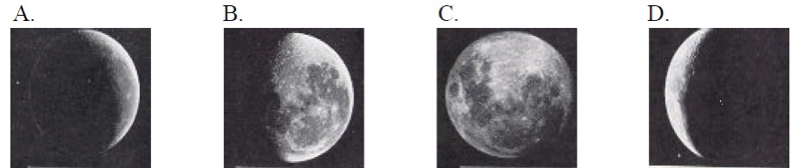
\includegraphics{asq10.png}
    \caption{}
    \label{fig:asq10}
\end{figure}
You observe a full Moon rising in the east. How will it appear in six hours? See Fig.~\ref{fig:asq10} for the options.
\begin{itemize}
    \item A
    \item B
    \item \underline{C}
    \item D
\end{itemize}
\item
In general, how confident are you that your answers to this survey are correct?
\begin{itemize}
    \item Not at all confident (just guessing)
    \item Not very confident
    \item Not sure
    \item Confident
    \item Very confident
\end{itemize}
\item
Which Astronomy Class are you signed up for?
\begin{itemize}
    \item Astronomy 100 (10936), TuTh at 10:00am
    \item Astronomy 100 (10937), TuTh at 1:00pm
    \item Astronomy 101 (23073), TuTh at 2:30pm
\end{itemize}
\item
What time zone do you call home?
\begin{itemize}
    \item Eastern
    \item Central
    \item Mountain
    \item Pacific
    \item Other: []
\end{itemize}
\item
What computer operating system do you use for homework?
\begin{itemize}
    \item Apple MacOS
    \item Microsoft Windows
    \item Apple iOS (e.g., iPad)
    \item Chromebook
    \item Linux
    \item Other: []
\end{itemize}
\item
For the purpose of the project this semester, what is the model of the phone or camera that you will be using? (Example: iPhone X, Samsung Galaxy S8, Nikon D3500 camera, etc.)

\textit{Note: you definitely do \textbf{not} need a state-of-the-art camera for these projects -- you just need to be able to take basic photos.}
\item
Over the course of these labs you will be taking pictures of sunsets (or sunrises) with your camera. To do this you will need to have access to a spot where you can view the western horizon for sunsets (eastern for sunrises). It's fine if these pictures are taken through a window.

\textbf{If you believe you need special accommodations for taking these photos or that the project will be impossible for you, please explain your circumstances below, and we will work out alternatives with you. (Otherwise, leave blank.)}
\end{enumerate}


\subsubsection{Quiz}

\begin{enumerate}
\item%TODO: ans
What was the approximate altitude of Jupiter at 6:00pm on January 31, 2022? \emph{(choose closest)}
\begin{itemize}
    \item 11°
    \item 34°
    \item 67°
    \item 145°
    \item 260°
\end{itemize}
\item
From the northern hemisphere, how do the azimuth and altitude of an object in the southeastern sky change with time?
\begin{itemize}
    \item Both decrease.
    \item \underline{Both increase.}
    \item The azimuth decreases while the altitude increase.
    \item The azimuth increases while the altitude decreases.
\end{itemize}
\item
From the northern hemisphere, how do the azimuth and altitude of an object in the southwestern sky change with time?
\begin{itemize}
    \item Both increase.
    \item Both decrease.
    \item The azimuth decreases while the altitude increases.
    \item \underline{The azimuth increases while the altitude decreases.}
\end{itemize}
\item
How do you predict the Sun's azimuth and altitude change as it sets in the western sky?
\begin{itemize}
    \item Unlike stars, it goes straight down, so its azimuth is constant.
    \item \underline{Its altitude and azimuth change much like those of any other setting star.}
    \item You can't measure altitudes or azimuths for the Sun.
\end{itemize}
\end{enumerate}


\newpage
\subsection{Lab 2: Angular Sizes on the Sky (equiv. to Project pt. 1)}

\subsubsection{Overview}

Topics covered:
\begin{itemize}
\item Estimating angular sizes and separations
\item Determining the field of view of your camera
\item Angles on the sky
\end{itemize}

\noindent
Watch out for:
\begin{itemize}
\item 
\end{itemize}


\subsubsection{Materials needed}

Instructors:
\begin{itemize}
\item Lab worksheets
\item Calibration grids
\end{itemize}

\noindent
Students:
\begin{itemize}
\item Fingers and arms
\item Camera
\end{itemize}


\subsubsection{Script}

\renewcommand\slidepath[1]{ppt/lab02/Slide#1.jpeg}

\emph{Before the end of class, set the Moodle Lab Quiz access password.}

\begin{longtable}{|m{0.5\textwidth}|m{0.5\textwidth}|}\hline
Pick up a copy of the lab worksheet. & \includegraphics[width=0.5\textwidth]{\slidepath{1}}\\\hline
Log in to Moodle and go to the Astronomy 100/101 Lab page. Review and respond to the Photo Policy Acknowledgement. You must respond in order to receive credit for this lab and the project.& \includegraphics[width=0.5\textwidth]{\slidepath{2}}\\\hline
We will use a uniform grid to get a sense of how to consistently compare the angular sizes we see. 

\begin{enumerate}
\item Stand with your eye/camera located 12 ft from the screen. 
\item Look at the floor plan to determine where you should stand. 
\item Sketch some things as they appear on the grid. 
\item Be consistent! E.g. if you are using 4 fingers at arm's length, always hold them out at full arm's length. 
\item Keep the worksheet to reference later about angular sizes.
\end{enumerate} & \includegraphics[width=0.5\textwidth]{\slidepath{3}}

\includegraphics[width=0.5\textwidth]{\slidepath{6}}\\\hline
Now we'll do the same with your camera to calibrate it.

\begin{enumerate}
\item Hold your camera at the same position as before, i.e. 12 ft from the screen.
\item Zoom in as far as you can on your camera.
\item Take a photo of the grid. Use the photo to determine the field of view of your camera.
\item Answer the questions on your worksheet.
\end{enumerate} & \includegraphics[width=0.5\textwidth]{\slidepath{7}}\\\hline
\begin{enumerate}
\item Look at the Stellarium view projected on the screens. It simulates a real-life view of the night sky at the same scale as the grid. 
\item Use similar things to those in Part 1 (fingers, coin, etc.) to estimate angular sizes and answer the questions on your worksheet. \textbf{Remember to be consistent! Hold your arm out at full length!}
\item Take a photo of the projected Moon like you did for the grid:
	\begin{itemize}
	\item Fully zoomed in
	\item Held at 12 ft from screen
	\end{itemize}
\item Answer the questions on your worksheet.
\end{enumerate}
 & \includegraphics[width=0.5\textwidth]{\slidepath{8}}

\includegraphics[width=0.5\textwidth]{\slidepath{9}}\\\hline
Now let's calibrate your camera fully zoomed out. 
\begin{enumerate}
\item Zoom out on your camera to 1x. \textbf{If your camera has 0.5x zoom or similar, do not use it.}
\item Take a photo of the grid from 12 ft. You'll see that the screen appears much smaller. Answer the question in the worksheet. 
\item Move your camera approximately 3 ft from the screen using a yardstick.  
\item Take a photo of the \text{new} grid, which has lines every 5deg. Use it to estimate the field of view of your camera fully zoomed out. Answer the questions on the worksheet.
\end{enumerate}
 & \includegraphics[width=0.5\textwidth]{\slidepath{10}}

\includegraphics[width=0.5\textwidth]{\slidepath{12}}\\\hline
Look at the Stellarium view projected on the screens. It simulates a real-life view shortly before sunset. 

\begin{enumerate}
\item With your camera 3 ft from the screen, take a photo of the screen.
\item Answer the questions in the worksheet and write them down for the quiz. 
\end{enumerate}

Take note that you will need to upload your calibration pictures on Moodle by the end of the week. 

If you switch to a new camera or change your settings, let your TAs know. There will be opportunities to re-calibrate your camera with the grids in future labs.
 & \includegraphics[width=0.5\textwidth]{\slidepath{13}}

\includegraphics[width=0.5\textwidth]{\slidepath{14}}\\\hline
\emph{At $\sim$ 10 min from class end, show Moodle quiz password.} 

Complete the Lab quiz on Moodle.

Remember to complete the pre-lab survey. & \includegraphics[width=0.5\textwidth]{\slidepath{21}}\\\hline
%\label{default}
\end{longtable}


\subsubsection{Submissions}

Moodle:
\begin{enumerate}
\item Lab quiz
\end{enumerate}

\noindent
In-class:
\begin{enumerate}
\item None
\end{enumerate}


\subsubsection{Quiz}

\begin{enumerate}
\item
What is the approximate angular size of the Moon?
\begin{itemize}
    \item \SI{0.2}{\degree}
    \item \underline{\SI{0.5}{\degree}}
    \item \SI{3}{\degree}
    \item \SI{8}{\degree}
    \item \SI{15}{\degree}
\end{itemize}
\item
What is the approximate angular separation between Aldebaran and the Pleiades?
\begin{itemize}
    \item \SI{0.2}{\degree}
    \item \SI{0.5}{\degree}
    \item \SI{3}{\degree}
    \item \SI{8}{\degree}
    \item \underline{\SI{15}{\degree}}
\end{itemize}
\item
Four billion years ago, the Moon was half as far away from Earth as it is now. What was the angular size of the Moon back then?
\begin{itemize}
    \item $2\times$ bigger
    \item \underline{$4\times$ bigger}
    \item $2\times$ smaller
    \item $4\times$ smaller
    \item the same 
\end{itemize}
\item
Suppose that you have an emergency and have to go home so you can't take your final sunset picture later in the semester. What should you do?
\begin{itemize}
    \item Try photoshopping the Sun on another picture you took
    \item Ask a friend to take the picture for you
    \item Use a friend's photo instead.
    \item Take a photo from home.
    \item \underline{Contact your lab instructor about what you might do instead.}
\end{itemize}
\item%TODO: answer
From the picture in part 3 of the lab, what were your estimates of the Sun's azimuth and altitude?
\begin{itemize}
    \item Azimuth: [$x$] \si{\degree} (enter a number only)
    \item Altitude: [$y$] \si{\degree} (enter a number only)
\end{itemize}
\end{enumerate}


\newpage
\subsection{Lab 3: Angular Size vs. Distance}

\subsubsection{Overview}

Topics covered:
\begin{itemize}
\item Observing angular size of an object at different distances
\item Interpreting the inverse relationship
\item The Sun’s angular size throughout the year
\end{itemize}

\noindent
Watch out for:
\begin{itemize}
\item 
\end{itemize}


\subsubsection{Materials needed}

Instructors:
\begin{itemize}
\item Lab worksheets
\item Volleyball/``volleyball"
\item Tripod/something to hold up volleyball e.g. lab stands $\times 3$
\item Blue tape to secure
\end{itemize}

\noindent
Students:
\begin{itemize}
\item 
\end{itemize}


\subsubsection{Script}

\renewcommand\slidepath[1]{ppt/lab03/Slide#1.jpeg}

\emph{Before the end of class, set the Moodle Lab Quiz access password.}

\begin{longtable}{|m{0.5\textwidth}|m{0.5\textwidth}|}\hline
Pick up a copy of the lab worksheet. Also, get a table worksheet for each table. & \includegraphics[width=0.5\textwidth]{\slidepath{1}}\\\hline
In groups at each table, you will investigate how the angular diameter of a spherical body (a ball) depends on its distance from you. Discuss and agree on a plan for how to make measurements of the sphere to explore the relationship between its angular size and distance. Make sure each person makes \textbf{at least one} measurement of the ball's angular size and distance. Consider:
\begin{enumerate}[a.]
\item What distances will you make measurements from?
\item How will you measure the distances?
\item Will you repeat the measurement with different people? (This is called replication.)
\item What will you do if points disagree?
\end{enumerate}
Record your measurement on both your lab and table worksheets. Then, mark and plot your points on the table worksheet.
 & \includegraphics[width=0.5\textwidth]{\slidepath{3}}\\\hline
Look over the points plotted by your group and discuss the following:
\begin{enumerate}
\item Do the points exhibit a pattern? How would you describe that pattern in words?
\item How might you describe the relationship mathematically?
\item Do all the points agree with each other? What factors might explain the differences we see?
\end{enumerate}
 & \includegraphics[width=0.5\textwidth]{\slidepath{4}}\\\hline
Here are two pictures of (half) the Sun taken with the same telescope and camera half a year apart. There's about a 2\% change in apparent diameter. Which picture was taken in January? Which in July? 
 & \includegraphics[width=0.5\textwidth]{\slidepath{5}}\\\hline
Now let's look at the Moon. What is the Moon's angular diameter? How much does that value change? Is it larger when it's full? What is a supermoon? 

Note that the Moon's angular diameter is actually SMALLER when it's close to the horizon because it's farther away than when it's high in the sky! It's a psychological illusion that the Moon feels larger near the horizon.
 & \includegraphics[width=0.5\textwidth]{\slidepath{6}}\\\hline
In groups of up to three,
\begin{enumerate}
\item Start up Stellarium and find Mars.
\item Turn off the atmosphere and ground visualisations.
\item Zoom in on Mars until Stellarium renders its features.
\item Note Mars's angular diameter in the left-side info panel.
\item Open the Date/Time window. 
\item Record and plot the angular diameter versus right ascension of Mars at least once per month from Oct 2021 to Oct 2023.
\end{enumerate}
 & \includegraphics[width=0.5\textwidth]{\slidepath{8}}\\\hline
Where is Mars this month? 

When Earth is closest to a planet and "passes" it, they appear to move backwards for a brief time, much like when you pass another car on the highway. This is called retrograde motion.
 & \includegraphics[width=0.5\textwidth]{\slidepath{9}}\\\hline
Up to few centuries ago, astronomers thought the Earth was the center of the solar system. They had to use epicycles to explain retrograde motion.
 & \includegraphics[width=0.5\textwidth]{\slidepath{10}}\\\hline
Fill out your worksheet.

\emph{At $\sim$ 10 min from class end, show Moodle quiz password.} 

Complete the Lab quiz on Moodle.

Remember to complete the pre-lab survey. & \includegraphics[width=0.5\textwidth]{\slidepath{11}}\\\hline
%\label{default}
\end{longtable}


\subsubsection{Submissions}

Moodle:
\begin{enumerate}
\item Lab quiz
\end{enumerate}

\noindent
In-class:
\begin{enumerate}
\item None
\end{enumerate}


\subsubsection{Quiz}

\begin{enumerate}
\item
What is your team's table number?
\begin{itemize}
    \item 1
    \item 2
    \item 3
    \item 4
    \item 5
    \item 6
    \item 7
    \item 8
    \item 9
    \item 10
    \item 11
\end{itemize}
\item
\begin{enumerate}[a.]
    \item When does Mars have the largest angular size?
    \begin{itemize}
        \item Oct 2021
        \item Nov 2021
        \item Dec 2021
        \item Jan 2022
        \item Feb 2022
        \item Mar 2022
        \item Apr 2022
        \item May 2022
        \item Jun 2022
        \item Jul 2022
        \item Aug 2022
        \item Sep 2022
        \item Oct 2022
        \item Nov 2022
        \item Dec 2022
        \item Jan 2023
        \item Feb 2023
        \item Mar 2023
        \item Apr 2023
        \item May 2023
        \item Jun 2023
        \item Jul 2023
        \item Aug 2023
        \item Sep 2023
        \item Oct 2023
    \end{itemize}
    \item What was its angular size in arcseconds? [\underline{\num{17(4)}}] \si{\arcsecond} (enter number only)
    \item Was it undergoing retrograde motion at this time? \underline{Yes}
\end{enumerate}
\item
Even though the Sun is physically much bigger than the Moon, they both have angular diameters of about \SI{0.5}{\degree}. This is because:
\begin{itemize}
    \item the Sun is so much brighter that we can’t look at it directly.
    \item the Moon has a solid surface, but the Sun is a transparent gas.
    \item \underline{the Sun is as many times farther away as it is larger.}
    \item our eyes cannot distinguish such small sizes, so they look the same.
    \item All of the above.
\end{itemize}
\item
Which of the following is a significant cause of Amherst’s summers being warmer than its winters?
\begin{itemize}
    \item Earth is closer to the Sun in the summer than in the winter.
    \item The northern hemisphere is closer to the Sun in the summer than in the winter.
    \item \underline{The ground faces the Sun more directly in the summer than in the winter.}
    \item All of the above.
\end{itemize}
\item
Suppose you see two friends across campus who you know are the same height as each other. Adam is \SI{2}{\degree} tall and Beth is \SI{6}{\degree} tall by your estimate.

Therefore, [\underline{Adam}] must be [\underline{3}] times \textbf{further away} from you.
\item
When does the Moon have the largest angular size?
\begin{itemize}
    \item When it is near the horizon.
    \item \underline{When it is in the part of its orbit closest to Earth.}
    \item When it is full
    \item When Earth is in the part of its orbit farthest from the Sun.
    \item All of the above.
\end{itemize}
\end{enumerate}


\newpage
\subsection{Lab 4: Phases of the Moon}

\subsubsection{Overview}

Topics covered:
\begin{itemize}
\item Relative size of Earth and Moon
\item Modelling phases
\item Relationship of moon phase to position in orbit and in our sky
\end{itemize}

\noindent
Watch out for:
\begin{itemize}
\item 
\end{itemize}


\subsubsection{Materials needed}

Instructors:
\begin{itemize}
\item Lab worksheets
\item Golf balls (box)
\item Lightbulbs on stands ($\times 11$)
\item Tape measure
\item Golf ball on stand
\end{itemize}

\noindent
Students:
\begin{itemize}
\item Computer
\end{itemize}


\subsubsection{Script}

Before the end of class, set the Moodle Lab Quiz access password.

\renewcommand\slidepath[1]{ppt/lab01/Slide#1.jpeg}
%\renewcommand\slidepath[1]{ppt/lab04/Slide#1.jpeg}

\emph{Before the end of class, set the Moodle Lab Quiz access password.}

\begin{longtable}{|m{0.5\textwidth}|m{0.5\textwidth}|}\hline
Pick up copies of lab worksheet, syllabus, and Stellarium guide. & \includegraphics[width=0.5\textwidth]{\slidepath{1}}\\\hline
Log in to Moodle, go to the Astronomy 100/101 Lab page, and fill out the Astronomy Background Survey. (The survey is graded on participation only.) & \includegraphics[width=0.5\textwidth]{\slidepath{3}}\\\hline
Astronomy Lab grade makes up 25\% of the Astronomy 100/101 total grade.

\textbf{Submitting work or pictures that are not your own, or having someone else do it for you, is dishonest and will be dealt with harshly.}

Lab usually improves your overall grade, if you put in the small time and effort commitment needed. & \includegraphics[width=0.5\textwidth]{\slidepath{5}}\\\hline
If you miss a lab, look out for at-home makeups or scheduled makeup labs, and try to let us know ASAP.

Don't procrastinate on the project; it's not difficult, but is impossible if left to the last minute. & \includegraphics[width=0.5\textwidth]{\slidepath{7}}\\\hline
Stellarium is a planetarium software that simulates what the sky looks like at different locations and times. & \includegraphics[width=0.5\textwidth]{\slidepath{8}}\\\hline
If you're using a lab computer, Stellarium is already installed and you can just pull it up. If you're using your own computer, download the correct installer from this website and install it. If your OS isn't available, you can use the web version. Open the Location Window from the left-hand menu panel or by pressing F6. In the search bar under the top right menu, type ``Amherst" and select ``Amherst Center, United States".

Take note that it's ``Amherst Center", not ``Amherst" (that's in NY somewhere). Also, \textbf{do not type} into the ``Name/City" box. That renames the location.

Close the window and open the Date/Time Window from the left-hand menu panel or by pressing F5. Set the time to 7:00pm tonight to see what will be visible.

Practice dragging the view with the cursor to view different directions. Note that to zoom in, you scroll \textbf{up}, and to zoom out, you scroll \textbf{down}. & \includegraphics[width=0.5\textwidth]{\slidepath{9}}\\\hline
In astronomy, we use angles to measure positions and separations of objects in the sky. Your position is measured by latitude and longitude. (These are angles measured with the vertex at the centre of the Earth. Where is the angle of your position measured relative to?) & \includegraphics[width=0.5\textwidth]{\slidepath{10}}\\\hline
From your point of view, an object's position is given by \textbf{azimuth} and \textbf{altitude}. Similar to before, we take the vertex of the angle measurement to be your position. For altitude, the angle is measured relative to the horizon. For azimuth, the angle is measured relative to due north. & \includegraphics[width=0.5\textwidth]{\slidepath{11}}\\\hline
To compare astronomical positions independent of observer location, we use the celestial coordinate system. It's very similar to latitude and longitude, which correcpond to declination and right ascension respectively. & \includegraphics[width=0.5\textwidth]{\slidepath{12}}\\\hline
Astronomers use the \textbf{sexagesimal} system for recording angles. Each degree is divided into 60 \textbf{arc minutes} (\si{\arcminute}), and each arc minute is divided into 60 \textbf{arc seconds} (\si{\arcsecond}).

Right ascension also measures angle, but it is measured like how we measure time, in hours-minutes-seconds. In right ascension, there are 24 hours in a circle of 360 \si{\degree}. & \includegraphics[width=0.5\textwidth]{\slidepath{13}}\\\hline
Fill out your worksheet. & \includegraphics[width=0.5\textwidth]{\slidepath{14}}\\\hline
%\emph{At ~10 min from class end, show Moodle quiz password.} 

%Complete the Lab quiz on Moodle.

Remember to complete the pre-lab survey. & \includegraphics[width=0.5\textwidth]{ppt/lab01/Slide15.jpeg}\\\hline
%\label{default}
\end{longtable}
%for instructors' table moon, some kind of tripod setup would be better
%need to clearly distinguish earth motion and moon motion


\subsubsection{Submissions}

Moodle:
\begin{enumerate}
\item Lab quiz
\end{enumerate}

\noindent
In-class:
\begin{enumerate}
\item None
\end{enumerate}


\subsubsection{Quiz}

\begin{enumerate}
\item
The Moon's shape appears to change over the course of each month because:
\begin{itemize}
    \item dark and bright spots come into view as the Moon rotates.
    \item parts of it become hidden as it passes into the Earth's shadow.
    \item \underline{the part of its sunlit side facing us depends on its orbital position.}
    \item the Moon's light is generated by internal volcanic processes.
\end{itemize}
\item
If we see the Moon is a crescent this evening from Amherst, what phase will it be when observed from Australia?
\begin{itemize}
    \item \underline{It will also be seen in the evening as a crescent.}
    \item It will appear to be nearly full.
    \item It will be seen as a crescent in the morning sky.
    \item The Moon can't be seen from Australia.
\end{itemize}
\item
If you see the Moon rising at about 9pm tonight, what time should you expect to see it rising a week from now?
\begin{itemize}
    \item 9pm
    \item \underline{3am}
    \item 9am
    \item 3pm
    \item None of these is correct-the Moon always rises at sunset.
\end{itemize}
\item
When can a lunar eclipse occur?
\begin{itemize}
    \item \underline{Only when the Moon is full.}
    \item Only when the Moon is new.
    \item When the Moon is at one of the quarter phases.
    \item At any phase but only at midnight.
\end{itemize}
\item%TODO: idk the answer
\begin{figure}[htbp]
    \centering
    \includegraphics{l4q5.png}
    \caption{}
    \label{fig:l4q5}
\end{figure}
In the image below (Fig.~\ref{fig:l4q5}), showing the Moon just above the eastern horizon, what is the phase of the Moon?
\begin{itemize}
    \item new
    \item first quarter
    \item full
    \item third (last) quarter
\end{itemize}
\item%TODO: idk the answer
In the same image as the previous question, about what time is it?
\begin{itemize}
    \item midnight
    \item sunrise
    \item noon
    \item sunset
\end{itemize}
\item
If it is a third quarter moon tonight, about how long will it be before the Moon is full?
\begin{itemize}
    \item A few days
    \item About a week
    \item About two weeks
    \item \underline{About 3 weeks}
    \item About a month
\end{itemize}
\item
When the Moon is gibbous, what phase would the Earth be in as seen from the Moon?
\begin{itemize}
    \item new
    \item \underline{crescent}
    \item quarter
    \item gibbous
    \item full
\end{itemize}
\end{enumerate}


\newpage
\subsection{Lab 5: Motions of the Sun}

\subsubsection{Overview}

Topics covered:
\begin{itemize}
\item The Sun’s altitude at noon throughout the year
\item The path of the Sun through the sky on different dates \item And at different latitudes
\end{itemize}

\noindent
Watch out for:
\begin{itemize}
\item 
\end{itemize}


\subsubsection{Materials needed}

Instructors:
\begin{itemize}
\item Lab worksheets
\end{itemize}

\noindent
Students:
\begin{itemize}
\item 
\end{itemize}


\subsubsection{Script}

%\renewcommand\slidepath[1]{ppt/lab05/Slide#1.jpeg}

\emph{Before the end of class, set the Moodle Lab Quiz access password.}

\begin{longtable}{|m{0.5\textwidth}|m{0.5\textwidth}|}\hline
Pick up copies of lab worksheet, syllabus, and Stellarium guide. & \includegraphics[width=0.5\textwidth]{\slidepath{1}}\\\hline
Log in to Moodle, go to the Astronomy 100/101 Lab page, and fill out the Astronomy Background Survey. (The survey is graded on participation only.) & \includegraphics[width=0.5\textwidth]{\slidepath{3}}\\\hline
Astronomy Lab grade makes up 25\% of the Astronomy 100/101 total grade.

\textbf{Submitting work or pictures that are not your own, or having someone else do it for you, is dishonest and will be dealt with harshly.}

Lab usually improves your overall grade, if you put in the small time and effort commitment needed. & \includegraphics[width=0.5\textwidth]{\slidepath{5}}\\\hline
If you miss a lab, look out for at-home makeups or scheduled makeup labs, and try to let us know ASAP.

Don't procrastinate on the project; it's not difficult, but is impossible if left to the last minute. & \includegraphics[width=0.5\textwidth]{\slidepath{7}}\\\hline
Stellarium is a planetarium software that simulates what the sky looks like at different locations and times. & \includegraphics[width=0.5\textwidth]{\slidepath{8}}\\\hline
If you're using a lab computer, Stellarium is already installed and you can just pull it up. If you're using your own computer, download the correct installer from this website and install it. If your OS isn't available, you can use the web version. Open the Location Window from the left-hand menu panel or by pressing F6. In the search bar under the top right menu, type ``Amherst" and select ``Amherst Center, United States".

Take note that it's ``Amherst Center", not ``Amherst" (that's in NY somewhere). Also, \textbf{do not type} into the ``Name/City" box. That renames the location.

Close the window and open the Date/Time Window from the left-hand menu panel or by pressing F5. Set the time to 7:00pm tonight to see what will be visible.

Practice dragging the view with the cursor to view different directions. Note that to zoom in, you scroll \textbf{up}, and to zoom out, you scroll \textbf{down}. & \includegraphics[width=0.5\textwidth]{\slidepath{9}}\\\hline
In astronomy, we use angles to measure positions and separations of objects in the sky. Your position is measured by latitude and longitude. (These are angles measured with the vertex at the centre of the Earth. Where is the angle of your position measured relative to?) & \includegraphics[width=0.5\textwidth]{\slidepath{10}}\\\hline
From your point of view, an object's position is given by \textbf{azimuth} and \textbf{altitude}. Similar to before, we take the vertex of the angle measurement to be your position. For altitude, the angle is measured relative to the horizon. For azimuth, the angle is measured relative to due north. & \includegraphics[width=0.5\textwidth]{\slidepath{11}}\\\hline
To compare astronomical positions independent of observer location, we use the celestial coordinate system. It's very similar to latitude and longitude, which correcpond to declination and right ascension respectively. & \includegraphics[width=0.5\textwidth]{\slidepath{12}}\\\hline
Astronomers use the \textbf{sexagesimal} system for recording angles. Each degree is divided into 60 \textbf{arc minutes} (\si{\arcminute}), and each arc minute is divided into 60 \textbf{arc seconds} (\si{\arcsecond}).

Right ascension also measures angle, but it is measured like how we measure time, in hours-minutes-seconds. In right ascension, there are 24 hours in a circle of 360 \si{\degree}. & \includegraphics[width=0.5\textwidth]{\slidepath{13}}\\\hline
Fill out your worksheet. & \includegraphics[width=0.5\textwidth]{\slidepath{14}}\\\hline
%\emph{At ~10 min from class end, show Moodle quiz password.} 

%Complete the Lab quiz on Moodle.

Remember to complete the pre-lab survey. & \includegraphics[width=0.5\textwidth]{ppt/lab01/Slide15.jpeg}\\\hline
%\label{default}
\end{longtable}
% the flow of this is so bad. need to smoothen flow. make each step have as little stellarium overhead as possible.


\subsubsection{Submissions}

Moodle:
\begin{enumerate}
\item Lab quiz
\end{enumerate}

\noindent
In-class:
\begin{enumerate}
\item None
\end{enumerate}


\subsubsection{Quiz}

\begin{enumerate}
\item
What is your table number?
\begin{itemize}
    \item 1
    \item 2
    \item 3
    \item 4
    \item 5
    \item 6
    \item 7
    \item 8
    \item 9
    \item 10
    \item 11
\end{itemize}
\item
\begin{enumerate}[a.]
    \item
    What is the latitude of your city in Section 2.b) of the worksheet? [$x$] \si{\degree} South (enter number only)
    \item
    At this location, what is the maximum altitude the Sun reaches during the year? [$y$] \si{\degree} (enter number only)
    \item
    At this location, what month does the Sun reach its maximum altitude at noon?
    \begin{itemize}
        \item January
        \item February
        \item March
        \item April
        \item May
        \item June
        \item July
        \item August
        \item September
        \item October
        \item November
        \item \underline{December}
    \end{itemize}
\end{enumerate}
\item
Where can you see the Sun pass straight overhead at noon? (see screen for options)
\begin{itemize}
    \item Everywhere on Earth.
    \item Everywhere between the arctic circles sometime during the year. 
    \item \underline{Everywhere within the topic latitudes sometime during the year.}
    \item Only on the equator.
    \item Nowhere on Earth.
\end{itemize}
\item
\begin{figure}[htbp]
    \centering
    \includegraphics{lab2_q4.png}
    \caption{}
    \label{fig:l5q4}
\end{figure}
If you were marooned on an island, and you saw a sunset angle as pictured below (Fig.~\ref{fig:l5q4}), what latitude would you likely be at?
\begin{itemize}
    \item N 60°
    \item N 30°
    \item 0°
    \item S 30°
    \item S 60°
\end{itemize}
\item
On what day does the Sun appear highest in the sky at noon in Amherst?
\begin{itemize}
    \item Vernal Equinox
    \item \underline{Summer Solstice}
    \item Autumnal Equinox
    \item Winter Solstice
\end{itemize}
\item
What month does the Sun appear highest in the sky at noon in Sydney, Australia (S \SI{34}{\degree})? (see screen for options)
\begin{itemize}
    \item March
    \item June
    \item September
    \item \underline{December} 
\end{itemize}
\end{enumerate}


\newpage
\subsection{Lab 6: Solar Power}

\subsubsection{Overview}

Topics covered:
\begin{itemize}
\item Experiments using flashlights to model the effect of distance on brightness of sunlight
\item The effect of angle
\item Solar heating and seasons
\end{itemize}

\noindent
Watch out for:
\begin{itemize}
\item 
\end{itemize}


\subsubsection{Materials needed}

Instructors:
\begin{itemize}
\item Lab worksheets
\item Table worksheets ($\times 11$)
\item Metre rules ($\times 11$)
\item Protractors ($\times 11$)
\item Flashlights ($\times 11$)
\end{itemize}

\noindent
Students:
\begin{itemize}
\item 
\end{itemize}


\subsubsection{Script}

%\renewcommand\slidepath[1]{ppt/lab06/Slide#1.jpeg}

\emph{Before the end of class, set the Moodle Lab Quiz access password.}

\begin{longtable}{|m{0.5\textwidth}|m{0.5\textwidth}|}\hline
Pick up copies of lab worksheet, syllabus, and Stellarium guide. & \includegraphics[width=0.5\textwidth]{\slidepath{1}}\\\hline
Log in to Moodle, go to the Astronomy 100/101 Lab page, and fill out the Astronomy Background Survey. (The survey is graded on participation only.) & \includegraphics[width=0.5\textwidth]{\slidepath{3}}\\\hline
Astronomy Lab grade makes up 25\% of the Astronomy 100/101 total grade.

\textbf{Submitting work or pictures that are not your own, or having someone else do it for you, is dishonest and will be dealt with harshly.}

Lab usually improves your overall grade, if you put in the small time and effort commitment needed. & \includegraphics[width=0.5\textwidth]{\slidepath{5}}\\\hline
If you miss a lab, look out for at-home makeups or scheduled makeup labs, and try to let us know ASAP.

Don't procrastinate on the project; it's not difficult, but is impossible if left to the last minute. & \includegraphics[width=0.5\textwidth]{\slidepath{7}}\\\hline
Stellarium is a planetarium software that simulates what the sky looks like at different locations and times. & \includegraphics[width=0.5\textwidth]{\slidepath{8}}\\\hline
If you're using a lab computer, Stellarium is already installed and you can just pull it up. If you're using your own computer, download the correct installer from this website and install it. If your OS isn't available, you can use the web version. Open the Location Window from the left-hand menu panel or by pressing F6. In the search bar under the top right menu, type ``Amherst" and select ``Amherst Center, United States".

Take note that it's ``Amherst Center", not ``Amherst" (that's in NY somewhere). Also, \textbf{do not type} into the ``Name/City" box. That renames the location.

Close the window and open the Date/Time Window from the left-hand menu panel or by pressing F5. Set the time to 7:00pm tonight to see what will be visible.

Practice dragging the view with the cursor to view different directions. Note that to zoom in, you scroll \textbf{up}, and to zoom out, you scroll \textbf{down}. & \includegraphics[width=0.5\textwidth]{\slidepath{9}}\\\hline
In astronomy, we use angles to measure positions and separations of objects in the sky. Your position is measured by latitude and longitude. (These are angles measured with the vertex at the centre of the Earth. Where is the angle of your position measured relative to?) & \includegraphics[width=0.5\textwidth]{\slidepath{10}}\\\hline
From your point of view, an object's position is given by \textbf{azimuth} and \textbf{altitude}. Similar to before, we take the vertex of the angle measurement to be your position. For altitude, the angle is measured relative to the horizon. For azimuth, the angle is measured relative to due north. & \includegraphics[width=0.5\textwidth]{\slidepath{11}}\\\hline
To compare astronomical positions independent of observer location, we use the celestial coordinate system. It's very similar to latitude and longitude, which correcpond to declination and right ascension respectively. & \includegraphics[width=0.5\textwidth]{\slidepath{12}}\\\hline
Astronomers use the \textbf{sexagesimal} system for recording angles. Each degree is divided into 60 \textbf{arc minutes} (\si{\arcminute}), and each arc minute is divided into 60 \textbf{arc seconds} (\si{\arcsecond}).

Right ascension also measures angle, but it is measured like how we measure time, in hours-minutes-seconds. In right ascension, there are 24 hours in a circle of 360 \si{\degree}. & \includegraphics[width=0.5\textwidth]{\slidepath{13}}\\\hline
Fill out your worksheet. & \includegraphics[width=0.5\textwidth]{\slidepath{14}}\\\hline
%\emph{At ~10 min from class end, show Moodle quiz password.} 

%Complete the Lab quiz on Moodle.

Remember to complete the pre-lab survey. & \includegraphics[width=0.5\textwidth]{ppt/lab01/Slide15.jpeg}\\\hline
%\label{default}
\end{longtable}


\subsubsection{Submissions}

Moodle:
\begin{enumerate}
\item Lab quiz
\end{enumerate}

\noindent
In-class:
\begin{enumerate}
\item Table worksheets
\end{enumerate}


\subsubsection{Quiz}

\begin{enumerate}
\item
What is your team's table number?
\begin{itemize}
    \item 1
    \item 2
    \item 3
    \item 4
    \item 5
    \item 6
    \item 7
    \item 8
    \item 9
    \item 10
    \item 11
\end{itemize}
\item
In what month is Earth closest to the Sun?
\begin{itemize}
    \item \underline{Jan}
    \item Feb
    \item Mar
    \item Apr
    \item May
    \item Jun
    \item Jul
    \item Aug
    \item Sep
    \item Oct
    \item Nov
    \item Dec
\end{itemize}
\item
When you double the distance from a light source, the intensity of the light:
\begin{itemize}
    \item \underline{gets 4 times smaller}
    \item gets 2 times smaller
    \item stays the same
    \item gets 2 times bigger
    \item gets 4 times bigger 
\end{itemize}
\item
Rate each of the following for its importance in explaining why we have cold temperatures in winter here in Amherst. There are three choices for each: important, unimportant/minor and has almost no effect, or works counter to the resulting temperature differences.
\begin{enumerate}[a.]
    \item Earth's Northern Hemisphere is farther from the Sun than the Southern Hemisphere. \underline{unimportant}
    \item Earth's orbit is elliptical and we get further away from the Sun in part of our orbit. \underline{counter}
    \item The angle of Earth's axis results in the Sun having a low altitude and its light spread out. \underline{important}
\end{enumerate}
\item
In part 3, what distance did your group estimate had the same intensity as light shining from an angle of 24°? [\underline{1.5}] ft (enter number only)
\item
List the values (last column in tables) your group measured at:
\begin{itemize}
    \item \SI{2.0}{ft} and \SI{90}{\degree}: [$x$] (enter number only)
    \item \SI{1.0}{ft} and \SI{47}{\degree}: [$y$] (enter number only)
\end{itemize}
\end{enumerate}


\newpage
\subsection{Lab 7: Calendars, Horoscopes, and Precession}% a.k.a. the fuck astrology lab}

\subsubsection{Overview}

Topics covered:
\begin{itemize}
\item Movement of the Sun and Moon through the zodiac
\item Understanding lunisolar calendars
\item What’s your sign?
\item Precession and the pole star
\end{itemize}

\noindent
Watch out for:
\begin{itemize}
\item 
\end{itemize}


\subsubsection{Materials needed}

Instructors:
\begin{itemize}
\item Lab worksheets
\end{itemize}

\noindent
Students:
\begin{itemize}
\item 
\end{itemize}


\subsubsection{Script}

%\renewcommand\slidepath[1]{ppt/lab07/Slide#1.jpeg}

\emph{Before the end of class, set the Moodle Lab Quiz access password.}

\begin{longtable}{|m{0.5\textwidth}|m{0.5\textwidth}|}\hline
Pick up copies of lab worksheet, syllabus, and Stellarium guide. & \includegraphics[width=0.5\textwidth]{\slidepath{1}}\\\hline
Log in to Moodle, go to the Astronomy 100/101 Lab page, and fill out the Astronomy Background Survey. (The survey is graded on participation only.) & \includegraphics[width=0.5\textwidth]{\slidepath{3}}\\\hline
Astronomy Lab grade makes up 25\% of the Astronomy 100/101 total grade.

\textbf{Submitting work or pictures that are not your own, or having someone else do it for you, is dishonest and will be dealt with harshly.}

Lab usually improves your overall grade, if you put in the small time and effort commitment needed. & \includegraphics[width=0.5\textwidth]{\slidepath{5}}\\\hline
If you miss a lab, look out for at-home makeups or scheduled makeup labs, and try to let us know ASAP.

Don't procrastinate on the project; it's not difficult, but is impossible if left to the last minute. & \includegraphics[width=0.5\textwidth]{\slidepath{7}}\\\hline
Stellarium is a planetarium software that simulates what the sky looks like at different locations and times. & \includegraphics[width=0.5\textwidth]{\slidepath{8}}\\\hline
If you're using a lab computer, Stellarium is already installed and you can just pull it up. If you're using your own computer, download the correct installer from this website and install it. If your OS isn't available, you can use the web version. Open the Location Window from the left-hand menu panel or by pressing F6. In the search bar under the top right menu, type ``Amherst" and select ``Amherst Center, United States".

Take note that it's ``Amherst Center", not ``Amherst" (that's in NY somewhere). Also, \textbf{do not type} into the ``Name/City" box. That renames the location.

Close the window and open the Date/Time Window from the left-hand menu panel or by pressing F5. Set the time to 7:00pm tonight to see what will be visible.

Practice dragging the view with the cursor to view different directions. Note that to zoom in, you scroll \textbf{up}, and to zoom out, you scroll \textbf{down}. & \includegraphics[width=0.5\textwidth]{\slidepath{9}}\\\hline
In astronomy, we use angles to measure positions and separations of objects in the sky. Your position is measured by latitude and longitude. (These are angles measured with the vertex at the centre of the Earth. Where is the angle of your position measured relative to?) & \includegraphics[width=0.5\textwidth]{\slidepath{10}}\\\hline
From your point of view, an object's position is given by \textbf{azimuth} and \textbf{altitude}. Similar to before, we take the vertex of the angle measurement to be your position. For altitude, the angle is measured relative to the horizon. For azimuth, the angle is measured relative to due north. & \includegraphics[width=0.5\textwidth]{\slidepath{11}}\\\hline
To compare astronomical positions independent of observer location, we use the celestial coordinate system. It's very similar to latitude and longitude, which correcpond to declination and right ascension respectively. & \includegraphics[width=0.5\textwidth]{\slidepath{12}}\\\hline
Astronomers use the \textbf{sexagesimal} system for recording angles. Each degree is divided into 60 \textbf{arc minutes} (\si{\arcminute}), and each arc minute is divided into 60 \textbf{arc seconds} (\si{\arcsecond}).

Right ascension also measures angle, but it is measured like how we measure time, in hours-minutes-seconds. In right ascension, there are 24 hours in a circle of 360 \si{\degree}. & \includegraphics[width=0.5\textwidth]{\slidepath{13}}\\\hline
Fill out your worksheet. & \includegraphics[width=0.5\textwidth]{\slidepath{14}}\\\hline
%\emph{At ~10 min from class end, show Moodle quiz password.} 

%Complete the Lab quiz on Moodle.

Remember to complete the pre-lab survey. & \includegraphics[width=0.5\textwidth]{ppt/lab01/Slide15.jpeg}\\\hline
%\label{default}
\end{longtable}


\subsubsection{Submissions}

Moodle:
\begin{enumerate}
\item Lab quiz
\end{enumerate}

\noindent
In-class:
\begin{enumerate}
\item None
\end{enumerate}


\subsubsection{Quiz}

\begin{enumerate}
\item
What determines that your horoscope sign is, for example, Taurus?
\begin{enumerate}[a.]
    \item Characteristics that are common among people born on those dates (like being bullish).
    \item The constellation (Taurus) the Moon is in on your birthday.
    \item The constellation (Taurus) the Sun is in on your birthday.
    \item \underline{None of the above.}
\end{enumerate}
\item
\begin{figure}[htbp]
    \centering
    \includegraphics{asq8.png}
    \caption{}
    \label{fig:l7q2}
\end{figure}
If you could see stars during the day, this is what the sky would look like at noon on a given day (Fig.~\ref{fig:l7q2}). The Sun is near the stars of the constellation Gemini. Near which constellation would you expect the Sun to be located at sunset?
\begin{enumerate}[a.]
    \item Leo
    \item Cancer
    \item \underline{Gemini}
    \item Taurus
    \item Pisces
\end{enumerate}
\item
For most people living today who, according to popular horoscopes, believe they are "a Gemini", the Sun was in the constellation [] on the day they were born.
\begin{enumerate}[a.]
    \item Leo
    \item \underline{Cancer}
    \item Gemini
    \item Taurus
    \item Pisces
\end{enumerate}
\item%TODO: ans?
Suppose it is just after sunset, and you see the constellation Gemini just above the horizon where the Sun set. If you were looking just after sunset a month later, what constellation would be in that position?
\begin{enumerate}[a.]
    \item Leo
    \item Cancer
    \item Gemini
    \item \underline{Taurus}
    \item Pisces
\end{enumerate}
\item
How many lunar months are there between Chinese New Years?
\begin{enumerate}[a.]
    \item 12
    \item 13
    \item 14
    \item \underline{12 or 13}
    \item 13 or 14
\end{enumerate}
\end{enumerate}


\newpage
\subsection{Lab 8: Motions of the Planets in the Sky}

\subsubsection{Overview}

Topics covered:
\begin{itemize}
\item Morning and evening stars
\item The motion of Mars
\item How retrograde motion varies among the planets
\end{itemize}

\noindent
Watch out for:
\begin{itemize}
\item 
\end{itemize}


\subsubsection{Materials needed}

Instructors:
\begin{itemize}
\item Lab worksheets
\end{itemize}

\noindent
Students:
\begin{itemize}
\item 
\end{itemize}


\subsubsection{Script}

%\renewcommand\slidepath[1]{ppt/lab08/Slide#1.jpeg}

\emph{Before the end of class, set the Moodle Lab Quiz access password.}

\begin{longtable}{|m{0.5\textwidth}|m{0.5\textwidth}|}\hline
Pick up copies of lab worksheet, syllabus, and Stellarium guide. & \includegraphics[width=0.5\textwidth]{\slidepath{1}}\\\hline
Log in to Moodle, go to the Astronomy 100/101 Lab page, and fill out the Astronomy Background Survey. (The survey is graded on participation only.) & \includegraphics[width=0.5\textwidth]{\slidepath{3}}\\\hline
Astronomy Lab grade makes up 25\% of the Astronomy 100/101 total grade.

\textbf{Submitting work or pictures that are not your own, or having someone else do it for you, is dishonest and will be dealt with harshly.}

Lab usually improves your overall grade, if you put in the small time and effort commitment needed. & \includegraphics[width=0.5\textwidth]{\slidepath{5}}\\\hline
If you miss a lab, look out for at-home makeups or scheduled makeup labs, and try to let us know ASAP.

Don't procrastinate on the project; it's not difficult, but is impossible if left to the last minute. & \includegraphics[width=0.5\textwidth]{\slidepath{7}}\\\hline
Stellarium is a planetarium software that simulates what the sky looks like at different locations and times. & \includegraphics[width=0.5\textwidth]{\slidepath{8}}\\\hline
If you're using a lab computer, Stellarium is already installed and you can just pull it up. If you're using your own computer, download the correct installer from this website and install it. If your OS isn't available, you can use the web version. Open the Location Window from the left-hand menu panel or by pressing F6. In the search bar under the top right menu, type ``Amherst" and select ``Amherst Center, United States".

Take note that it's ``Amherst Center", not ``Amherst" (that's in NY somewhere). Also, \textbf{do not type} into the ``Name/City" box. That renames the location.

Close the window and open the Date/Time Window from the left-hand menu panel or by pressing F5. Set the time to 7:00pm tonight to see what will be visible.

Practice dragging the view with the cursor to view different directions. Note that to zoom in, you scroll \textbf{up}, and to zoom out, you scroll \textbf{down}. & \includegraphics[width=0.5\textwidth]{\slidepath{9}}\\\hline
In astronomy, we use angles to measure positions and separations of objects in the sky. Your position is measured by latitude and longitude. (These are angles measured with the vertex at the centre of the Earth. Where is the angle of your position measured relative to?) & \includegraphics[width=0.5\textwidth]{\slidepath{10}}\\\hline
From your point of view, an object's position is given by \textbf{azimuth} and \textbf{altitude}. Similar to before, we take the vertex of the angle measurement to be your position. For altitude, the angle is measured relative to the horizon. For azimuth, the angle is measured relative to due north. & \includegraphics[width=0.5\textwidth]{\slidepath{11}}\\\hline
To compare astronomical positions independent of observer location, we use the celestial coordinate system. It's very similar to latitude and longitude, which correcpond to declination and right ascension respectively. & \includegraphics[width=0.5\textwidth]{\slidepath{12}}\\\hline
Astronomers use the \textbf{sexagesimal} system for recording angles. Each degree is divided into 60 \textbf{arc minutes} (\si{\arcminute}), and each arc minute is divided into 60 \textbf{arc seconds} (\si{\arcsecond}).

Right ascension also measures angle, but it is measured like how we measure time, in hours-minutes-seconds. In right ascension, there are 24 hours in a circle of 360 \si{\degree}. & \includegraphics[width=0.5\textwidth]{\slidepath{13}}\\\hline
Fill out your worksheet. & \includegraphics[width=0.5\textwidth]{\slidepath{14}}\\\hline
%\emph{At ~10 min from class end, show Moodle quiz password.} 

%Complete the Lab quiz on Moodle.

Remember to complete the pre-lab survey. & \includegraphics[width=0.5\textwidth]{ppt/lab01/Slide15.jpeg}\\\hline
%\label{default}
\end{longtable}


\subsubsection{Submissions}

Moodle:
\begin{enumerate}
\item Lab quiz
\end{enumerate}

\noindent
In-class:
\begin{enumerate}
\item None
\end{enumerate}


\subsubsection{Quiz}

\begin{enumerate}
\item
When is Mars brightest?
\begin{enumerate}[a.]
    \item Just at the beginning or end of retrograde motion, when Mars appears stationary.
    \item In July, when Earth is farthest from the Sun.
    \item When it is on the far side of the Sun, so we see its fully-lit face.
    \item \underline{In the middle of going through retrograde motion.}
\end{enumerate}
\item
Which planets undergo retrograde (backward) motion on the sky?
\begin{enumerate}[a.]
    \item Mars only.
    \item Just Mars, Jupiter, Saturn, Uranus, and Neptune.
    \item Venus only.
    \item Just Venus and Mercury.
    \item \underline{All of the planets.}
\end{enumerate}
\end{enumerate}


\newpage
\subsection{Lab 9: The HR Diagram}

\subsubsection{Overview}

Topics covered:
\begin{itemize}
\item Stellar temperatures and luminosities from colour and magnitude
\item Finding stellar radii
\item Bright stars vs. nearby stars
\end{itemize}

\noindent
Watch out for:
\begin{itemize}
\item 
\end{itemize}


\subsubsection{Materials needed}

Instructors:
\begin{itemize}
  \item Lab worksheets
  \item Table worksheets ($\times 11$)
\end{itemize}

\noindent
Students:
\begin{itemize}
  \item 
\end{itemize}


\subsubsection{Script}

%\renewcommand\slidepath[1]{ppt/lab09/Slide#1.jpeg}

\emph{Before the end of class, set the Moodle Lab Quiz access password.}

\begin{longtable}{|m{0.5\textwidth}|m{0.5\textwidth}|}\hline
Pick up copies of lab worksheet, syllabus, and Stellarium guide. & \includegraphics[width=0.5\textwidth]{\slidepath{1}}\\\hline
Log in to Moodle, go to the Astronomy 100/101 Lab page, and fill out the Astronomy Background Survey. (The survey is graded on participation only.) & \includegraphics[width=0.5\textwidth]{\slidepath{3}}\\\hline
Astronomy Lab grade makes up 25\% of the Astronomy 100/101 total grade.

\textbf{Submitting work or pictures that are not your own, or having someone else do it for you, is dishonest and will be dealt with harshly.}

Lab usually improves your overall grade, if you put in the small time and effort commitment needed. & \includegraphics[width=0.5\textwidth]{\slidepath{5}}\\\hline
If you miss a lab, look out for at-home makeups or scheduled makeup labs, and try to let us know ASAP.

Don't procrastinate on the project; it's not difficult, but is impossible if left to the last minute. & \includegraphics[width=0.5\textwidth]{\slidepath{7}}\\\hline
Stellarium is a planetarium software that simulates what the sky looks like at different locations and times. & \includegraphics[width=0.5\textwidth]{\slidepath{8}}\\\hline
If you're using a lab computer, Stellarium is already installed and you can just pull it up. If you're using your own computer, download the correct installer from this website and install it. If your OS isn't available, you can use the web version. Open the Location Window from the left-hand menu panel or by pressing F6. In the search bar under the top right menu, type ``Amherst" and select ``Amherst Center, United States".

Take note that it's ``Amherst Center", not ``Amherst" (that's in NY somewhere). Also, \textbf{do not type} into the ``Name/City" box. That renames the location.

Close the window and open the Date/Time Window from the left-hand menu panel or by pressing F5. Set the time to 7:00pm tonight to see what will be visible.

Practice dragging the view with the cursor to view different directions. Note that to zoom in, you scroll \textbf{up}, and to zoom out, you scroll \textbf{down}. & \includegraphics[width=0.5\textwidth]{\slidepath{9}}\\\hline
In astronomy, we use angles to measure positions and separations of objects in the sky. Your position is measured by latitude and longitude. (These are angles measured with the vertex at the centre of the Earth. Where is the angle of your position measured relative to?) & \includegraphics[width=0.5\textwidth]{\slidepath{10}}\\\hline
From your point of view, an object's position is given by \textbf{azimuth} and \textbf{altitude}. Similar to before, we take the vertex of the angle measurement to be your position. For altitude, the angle is measured relative to the horizon. For azimuth, the angle is measured relative to due north. & \includegraphics[width=0.5\textwidth]{\slidepath{11}}\\\hline
To compare astronomical positions independent of observer location, we use the celestial coordinate system. It's very similar to latitude and longitude, which correcpond to declination and right ascension respectively. & \includegraphics[width=0.5\textwidth]{\slidepath{12}}\\\hline
Astronomers use the \textbf{sexagesimal} system for recording angles. Each degree is divided into 60 \textbf{arc minutes} (\si{\arcminute}), and each arc minute is divided into 60 \textbf{arc seconds} (\si{\arcsecond}).

Right ascension also measures angle, but it is measured like how we measure time, in hours-minutes-seconds. In right ascension, there are 24 hours in a circle of 360 \si{\degree}. & \includegraphics[width=0.5\textwidth]{\slidepath{13}}\\\hline
Fill out your worksheet. & \includegraphics[width=0.5\textwidth]{\slidepath{14}}\\\hline
%\emph{At ~10 min from class end, show Moodle quiz password.} 

%Complete the Lab quiz on Moodle.

Remember to complete the pre-lab survey. & \includegraphics[width=0.5\textwidth]{ppt/lab01/Slide15.jpeg}\\\hline
%\label{default}
\end{longtable}


\subsubsection{Submissions}

Moodle:
\begin{enumerate}
\item Lab quiz
\end{enumerate}

\noindent
In-class:
\begin{enumerate}
\item Table worksheets
\end{enumerate}


\subsubsection{Quiz}

\begin{enumerate}
\item
What is your team's table number?
\begin{itemize}
    \item 1
    \item 2
    \item 3
    \item 4
    \item 5
    \item 6
    \item 7
    \item 8
    \item 9
    \item 10
    \item 11
\end{itemize}
\item
Enter the data you found for your bright star. (enter number only)

Distance: [$d$] ly (light-years)

Temperature: [$T$] K (Kelvin)

Size: [$D$] $\times$ diameter of Sun
\item
Which of the following is true about the Sun? (select all that apply)
\begin{itemize}
    \item \underline{The Sun is a star.}
    \item The Sun is bigger than most stars.
    \item The Sun is more luminous than most stars.
    \item \underline{The Sun is less luminous than most of the brightest stars we see at night.}
\end{itemize}
\item
Which of the following is true about the brightest stars you can see by eye at night? (select one)
\begin{itemize}
    \item \underline{Most are giant stars, much more luminous than the Sun.}
    \item Most are very nearby, making them look so bright.
    \item Most are small, red stars, which are the most common.%TODO: phrasing
    \item Most are young, so they have a lot of fuel to burn.
\end{itemize}
\item
What does absolute magnitude measure?
\begin{itemize}
    \item A star's distance in parsecs.
    \item How bright a star appears to be.
    \item The brightness of a star if observed from above Earth's atmosphere.
    \item \underline{The power output from a star in starlight.}
\end{itemize}
\item
Which of the following would you need to know to find a star's surface temperature? (select all that apply)
\begin{itemize}
    \item Distance to star
    \item Radius of star
    \item Absolute magnitude of star
    \item \underline{B-V color of star}
\end{itemize}
\end{enumerate}


\newpage
\subsection{Lab 10: Distances of Stars in Space}

\subsubsection{Overview}

Topics covered:
\begin{itemize}
\item Building a 3D constellation
\item Understanding spectral type and luminosity class
\item Understanding parallax
\end{itemize}

\noindent
Watch out for:
\begin{itemize}
\item 
\end{itemize}


\subsubsection{Materials needed}

Instructors:
\begin{itemize}
\item Lab worksheets
\item Table worksheets ($\times 11$)
\item Tribbles (in box)
\item Clips (in box)
\item Metal poles with sightlines ($\times 11$)
\end{itemize}

\noindent
Students:
\begin{itemize}
\item 
\end{itemize}


\subsubsection{Script}

%\renewcommand\slidepath[1]{ppt/lab10/Slide#1.jpeg}

\emph{Before the end of class, set the Moodle Lab Quiz access password.}

\begin{longtable}{|m{0.5\textwidth}|m{0.5\textwidth}|}\hline
Pick up copies of lab worksheet, syllabus, and Stellarium guide. & \includegraphics[width=0.5\textwidth]{\slidepath{1}}\\\hline
Log in to Moodle, go to the Astronomy 100/101 Lab page, and fill out the Astronomy Background Survey. (The survey is graded on participation only.) & \includegraphics[width=0.5\textwidth]{\slidepath{3}}\\\hline
Astronomy Lab grade makes up 25\% of the Astronomy 100/101 total grade.

\textbf{Submitting work or pictures that are not your own, or having someone else do it for you, is dishonest and will be dealt with harshly.}

Lab usually improves your overall grade, if you put in the small time and effort commitment needed. & \includegraphics[width=0.5\textwidth]{\slidepath{5}}\\\hline
If you miss a lab, look out for at-home makeups or scheduled makeup labs, and try to let us know ASAP.

Don't procrastinate on the project; it's not difficult, but is impossible if left to the last minute. & \includegraphics[width=0.5\textwidth]{\slidepath{7}}\\\hline
Stellarium is a planetarium software that simulates what the sky looks like at different locations and times. & \includegraphics[width=0.5\textwidth]{\slidepath{8}}\\\hline
If you're using a lab computer, Stellarium is already installed and you can just pull it up. If you're using your own computer, download the correct installer from this website and install it. If your OS isn't available, you can use the web version. Open the Location Window from the left-hand menu panel or by pressing F6. In the search bar under the top right menu, type ``Amherst" and select ``Amherst Center, United States".

Take note that it's ``Amherst Center", not ``Amherst" (that's in NY somewhere). Also, \textbf{do not type} into the ``Name/City" box. That renames the location.

Close the window and open the Date/Time Window from the left-hand menu panel or by pressing F5. Set the time to 7:00pm tonight to see what will be visible.

Practice dragging the view with the cursor to view different directions. Note that to zoom in, you scroll \textbf{up}, and to zoom out, you scroll \textbf{down}. & \includegraphics[width=0.5\textwidth]{\slidepath{9}}\\\hline
In astronomy, we use angles to measure positions and separations of objects in the sky. Your position is measured by latitude and longitude. (These are angles measured with the vertex at the centre of the Earth. Where is the angle of your position measured relative to?) & \includegraphics[width=0.5\textwidth]{\slidepath{10}}\\\hline
From your point of view, an object's position is given by \textbf{azimuth} and \textbf{altitude}. Similar to before, we take the vertex of the angle measurement to be your position. For altitude, the angle is measured relative to the horizon. For azimuth, the angle is measured relative to due north. & \includegraphics[width=0.5\textwidth]{\slidepath{11}}\\\hline
To compare astronomical positions independent of observer location, we use the celestial coordinate system. It's very similar to latitude and longitude, which correcpond to declination and right ascension respectively. & \includegraphics[width=0.5\textwidth]{\slidepath{12}}\\\hline
Astronomers use the \textbf{sexagesimal} system for recording angles. Each degree is divided into 60 \textbf{arc minutes} (\si{\arcminute}), and each arc minute is divided into 60 \textbf{arc seconds} (\si{\arcsecond}).

Right ascension also measures angle, but it is measured like how we measure time, in hours-minutes-seconds. In right ascension, there are 24 hours in a circle of 360 \si{\degree}. & \includegraphics[width=0.5\textwidth]{\slidepath{13}}\\\hline
Fill out your worksheet. & \includegraphics[width=0.5\textwidth]{\slidepath{14}}\\\hline
%\emph{At ~10 min from class end, show Moodle quiz password.} 

%Complete the Lab quiz on Moodle.

Remember to complete the pre-lab survey. & \includegraphics[width=0.5\textwidth]{ppt/lab01/Slide15.jpeg}\\\hline
%\label{default}
\end{longtable}


\subsubsection{Submissions}

Moodle:
\begin{enumerate}
\item Lab quiz
\end{enumerate}

\noindent
In-class:
\begin{enumerate}
\item Table worksheets
\end{enumerate}


\subsubsection{Quiz}

\begin{enumerate}
\item
What is your team's table number?
\begin{itemize}
    \item 1
    \item 2
    \item 3
    \item 4
    \item 5
    \item 6
    \item 7
    \item 8
    \item 9
    \item 10
    \item 11
\end{itemize}
\item
What constellation did your table work on?
\item
Light from the Sun takes about 8.5 minutes to reach Earth. About how long does light take to reach us from most of the brighter stars we see at night?
\begin{itemize}
    \item Several hours
    \item Several months
    \item 3-10 years
    \item \underline{100-1000 years}
    \item Millions of years
\end{itemize}
\item
Most constellations are collections of stars that:
\begin{itemize}
    \item \underline{are not physically associated with each other.}
    \item are members of a group of stars gravitationally attracted together.
    \item were born together out of a cloud of gas, now drifting apart.
    \item were born out of the same interstellar cloud as the Sun.
\end{itemize}
\item
Suppose star A has a parallax shift 10 times larger than star B. Which of the following is true?
\begin{itemize}
    \item \underline{Star A is 10 times closer than star B.}
    \item Star A is 10 times farther than star B.
    \item Star A is 100 times closer than star B.
    \item Star A is 100 times farther than star B.
\end{itemize}
\item
If you spot a bright reddish colored star in a constellation tonight, it is most probably:
\begin{itemize}
    \item \underline{a distant red giant star.}
    \item a nearby low-mass main-sequence star.
    \item either A or B with about equal probability.
\end{itemize}
\item
As viewed from Massachusetts, the stars of the Big Dipper can be connected with imaginary lines to form the shape of a bowl with a curved handle. What is the closest point you would have to travel to in order to observe a substantial change in the shape formed by these stars?
\begin{itemize}
    \item Across the country
    \item Another continent
    \item The Moon
    \item Pluto
    \item \underline{A distant star}
\end{itemize}
\item
If you lived on Mars, how would the parallax of stars differ from its value seen from Earth?
\begin{itemize}
    \item \underline{It would be bigger.}
    \item It would be smaller.
    \item It would be the same.
\end{itemize}
\end{enumerate}


\newpage
\subsection{Lab 11: Structure of the Local Group}

\subsubsection{Overview}

Topics covered:
\begin{itemize}
\item Using angular sizes to estimate nearby galaxy sizes
\item Building a scale model of the Local Group of galaxies
\end{itemize}

\noindent
Watch out for:
\begin{itemize}
\item 
\end{itemize}


\subsubsection{Materials needed}

Instructors:
\begin{itemize}
\item Lab worksheets
\item Colour paper (green, yellow, blue)
\item Scissors (multiple)
\item Galaxy info strips
\item Milky Way scale paper disc
\item Tripod/chair/something to put the Milky Way on e.g. lab stand
\end{itemize}

\noindent
Students:
\begin{itemize}
\item 
\end{itemize}


\subsubsection{Script}

%\renewcommand\slidepath[1]{ppt/lab11/Slide#1.jpeg}

\emph{Before the end of class, set the Moodle Lab Quiz access password.}

\begin{longtable}{|m{0.5\textwidth}|m{0.5\textwidth}|}\hline
Pick up copies of lab worksheet, syllabus, and Stellarium guide. & \includegraphics[width=0.5\textwidth]{\slidepath{1}}\\\hline
Log in to Moodle, go to the Astronomy 100/101 Lab page, and fill out the Astronomy Background Survey. (The survey is graded on participation only.) & \includegraphics[width=0.5\textwidth]{\slidepath{3}}\\\hline
Astronomy Lab grade makes up 25\% of the Astronomy 100/101 total grade.

\textbf{Submitting work or pictures that are not your own, or having someone else do it for you, is dishonest and will be dealt with harshly.}

Lab usually improves your overall grade, if you put in the small time and effort commitment needed. & \includegraphics[width=0.5\textwidth]{\slidepath{5}}\\\hline
If you miss a lab, look out for at-home makeups or scheduled makeup labs, and try to let us know ASAP.

Don't procrastinate on the project; it's not difficult, but is impossible if left to the last minute. & \includegraphics[width=0.5\textwidth]{\slidepath{7}}\\\hline
Stellarium is a planetarium software that simulates what the sky looks like at different locations and times. & \includegraphics[width=0.5\textwidth]{\slidepath{8}}\\\hline
If you're using a lab computer, Stellarium is already installed and you can just pull it up. If you're using your own computer, download the correct installer from this website and install it. If your OS isn't available, you can use the web version. Open the Location Window from the left-hand menu panel or by pressing F6. In the search bar under the top right menu, type ``Amherst" and select ``Amherst Center, United States".

Take note that it's ``Amherst Center", not ``Amherst" (that's in NY somewhere). Also, \textbf{do not type} into the ``Name/City" box. That renames the location.

Close the window and open the Date/Time Window from the left-hand menu panel or by pressing F5. Set the time to 7:00pm tonight to see what will be visible.

Practice dragging the view with the cursor to view different directions. Note that to zoom in, you scroll \textbf{up}, and to zoom out, you scroll \textbf{down}. & \includegraphics[width=0.5\textwidth]{\slidepath{9}}\\\hline
In astronomy, we use angles to measure positions and separations of objects in the sky. Your position is measured by latitude and longitude. (These are angles measured with the vertex at the centre of the Earth. Where is the angle of your position measured relative to?) & \includegraphics[width=0.5\textwidth]{\slidepath{10}}\\\hline
From your point of view, an object's position is given by \textbf{azimuth} and \textbf{altitude}. Similar to before, we take the vertex of the angle measurement to be your position. For altitude, the angle is measured relative to the horizon. For azimuth, the angle is measured relative to due north. & \includegraphics[width=0.5\textwidth]{\slidepath{11}}\\\hline
To compare astronomical positions independent of observer location, we use the celestial coordinate system. It's very similar to latitude and longitude, which correcpond to declination and right ascension respectively. & \includegraphics[width=0.5\textwidth]{\slidepath{12}}\\\hline
Astronomers use the \textbf{sexagesimal} system for recording angles. Each degree is divided into 60 \textbf{arc minutes} (\si{\arcminute}), and each arc minute is divided into 60 \textbf{arc seconds} (\si{\arcsecond}).

Right ascension also measures angle, but it is measured like how we measure time, in hours-minutes-seconds. In right ascension, there are 24 hours in a circle of 360 \si{\degree}. & \includegraphics[width=0.5\textwidth]{\slidepath{13}}\\\hline
Fill out your worksheet. & \includegraphics[width=0.5\textwidth]{\slidepath{14}}\\\hline
%\emph{At ~10 min from class end, show Moodle quiz password.} 

%Complete the Lab quiz on Moodle.

Remember to complete the pre-lab survey. & \includegraphics[width=0.5\textwidth]{ppt/lab01/Slide15.jpeg}\\\hline
%\label{default}
\end{longtable}


\subsubsection{Submissions}

Moodle:
\begin{enumerate}
\item Lab quiz
\item Astronomy post-instruction survey
\end{enumerate}

\noindent
In-class:
\begin{enumerate}
\item None
\end{enumerate}


\subsubsection{Quiz}

\begin{enumerate}
\item
What is the number of the galaxy you worked on?
\item
What was the distance of your galaxy (in light years)? [$d$] ly (enter number only)
\item
What diameter did you estimate for your galaxy (in light years)? [$D$] ly (enter number only)
\item
Approximately how far away is the nearest galaxy that is the size of the Milky Way or larger?
\begin{itemize}
    \item About 25,000 light years
    \item \underline{About 2,500,000 light years}
    \item About 250,000,000 light years
    \item About 2,500,000,000 light years
\end{itemize}
\item
What is the most common type of galaxy in the Local Group of galaxies?
\begin{itemize}
    \item Spiral
    \item Elliptical
    \item Irregular
    \item \underline{Dwarf}
\end{itemize}
\item
What information is needed to find the physical diameter of a galaxy? (select only those items that are necessary)
\begin{itemize}
    \item \underline{Angular diameter}
    \item \underline{Distance}
    \item Classification
    \item Magnitude
    \item Color
\end{itemize}
\item
Which of the following best describes the Milky Way galaxy as compared to the other galaxies in the Local Group?
\begin{itemize}
    \item \underline{One of the largest galaxies in the Local Group.}
    \item One of the smaller galaxies in the Local Group.
    \item The only spiral galaxy in the Local Group.
    \item The only large galaxy in the Local Group.
    \item One of the only dwarf galaxies in the Local Group.
\end{itemize}
\end{enumerate}


\newpage
\subsection{Project: Movement of the Sunset}

\subsubsection{Overview}

Topics covered:
\begin{itemize}
\item 
\end{itemize}

\noindent
Watch out for:
\begin{itemize}
\item 
\end{itemize}


\subsubsection{Materials needed}

Instructors:
\begin{itemize}
\item Calibration grids
\end{itemize}

\noindent
Students:
\begin{itemize}
\item Camera
\end{itemize}


\subsubsection{Script}

%\renewcommand\slidepath[1]{ppt/proj/Slide#1.jpeg}

\emph{Before the end of class, set the Moodle Lab Quiz access password.}

\begin{longtable}{|m{0.5\textwidth}|m{0.5\textwidth}|}\hline
Pick up copies of lab worksheet, syllabus, and Stellarium guide. & \includegraphics[width=0.5\textwidth]{\slidepath{1}}\\\hline
Log in to Moodle, go to the Astronomy 100/101 Lab page, and fill out the Astronomy Background Survey. (The survey is graded on participation only.) & \includegraphics[width=0.5\textwidth]{\slidepath{3}}\\\hline
Astronomy Lab grade makes up 25\% of the Astronomy 100/101 total grade.

\textbf{Submitting work or pictures that are not your own, or having someone else do it for you, is dishonest and will be dealt with harshly.}

Lab usually improves your overall grade, if you put in the small time and effort commitment needed. & \includegraphics[width=0.5\textwidth]{\slidepath{5}}\\\hline
If you miss a lab, look out for at-home makeups or scheduled makeup labs, and try to let us know ASAP.

Don't procrastinate on the project; it's not difficult, but is impossible if left to the last minute. & \includegraphics[width=0.5\textwidth]{\slidepath{7}}\\\hline
Stellarium is a planetarium software that simulates what the sky looks like at different locations and times. & \includegraphics[width=0.5\textwidth]{\slidepath{8}}\\\hline
If you're using a lab computer, Stellarium is already installed and you can just pull it up. If you're using your own computer, download the correct installer from this website and install it. If your OS isn't available, you can use the web version. Open the Location Window from the left-hand menu panel or by pressing F6. In the search bar under the top right menu, type ``Amherst" and select ``Amherst Center, United States".

Take note that it's ``Amherst Center", not ``Amherst" (that's in NY somewhere). Also, \textbf{do not type} into the ``Name/City" box. That renames the location.

Close the window and open the Date/Time Window from the left-hand menu panel or by pressing F5. Set the time to 7:00pm tonight to see what will be visible.

Practice dragging the view with the cursor to view different directions. Note that to zoom in, you scroll \textbf{up}, and to zoom out, you scroll \textbf{down}. & \includegraphics[width=0.5\textwidth]{\slidepath{9}}\\\hline
In astronomy, we use angles to measure positions and separations of objects in the sky. Your position is measured by latitude and longitude. (These are angles measured with the vertex at the centre of the Earth. Where is the angle of your position measured relative to?) & \includegraphics[width=0.5\textwidth]{\slidepath{10}}\\\hline
From your point of view, an object's position is given by \textbf{azimuth} and \textbf{altitude}. Similar to before, we take the vertex of the angle measurement to be your position. For altitude, the angle is measured relative to the horizon. For azimuth, the angle is measured relative to due north. & \includegraphics[width=0.5\textwidth]{\slidepath{11}}\\\hline
To compare astronomical positions independent of observer location, we use the celestial coordinate system. It's very similar to latitude and longitude, which correcpond to declination and right ascension respectively. & \includegraphics[width=0.5\textwidth]{\slidepath{12}}\\\hline
Astronomers use the \textbf{sexagesimal} system for recording angles. Each degree is divided into 60 \textbf{arc minutes} (\si{\arcminute}), and each arc minute is divided into 60 \textbf{arc seconds} (\si{\arcsecond}).

Right ascension also measures angle, but it is measured like how we measure time, in hours-minutes-seconds. In right ascension, there are 24 hours in a circle of 360 \si{\degree}. & \includegraphics[width=0.5\textwidth]{\slidepath{13}}\\\hline
Fill out your worksheet. & \includegraphics[width=0.5\textwidth]{\slidepath{14}}\\\hline
%\emph{At ~10 min from class end, show Moodle quiz password.} 

%Complete the Lab quiz on Moodle.

Remember to complete the pre-lab survey. & \includegraphics[width=0.5\textwidth]{ppt/lab01/Slide15.jpeg}\\\hline
%\label{default}
\end{longtable}


\subsubsection{Photo Policy Acknowledgement}

You will need to take several photos of the setting Sun over the course of the semester following specific directions. Taking these photos is not difficult, but it does require some advance planning. Picture requirements will be described in lab and on Moodle, but a cell phone camera is fine.

You will need to upload your own original pictures taken this semester into Moodle over the course of the semester. Submitting pictures you didn't take yourself this semester, or helping someone else to submit pictures that are not their own, is considered plagiarism and/or academic dishonesty and will be handled in accordance with the UMass Academic Honesty Policy, and may result in penalties up to a zero for the entire project.

You are responsible for saving backups of your pictures immediately, so a lost or broken phone/camera/computer is not an excuse for failing to submit your pictures on time. You can upload your pictures into Moodle as you take them and save backups of your pictures using UMass OneDrive, for example.

If you have any special circumstances that will not allow you to take sunset photos for your project. You must contact your lab instructor right away to explain the circumstances and come to alternative arrangements with them.

Please indicate that you understand these policies by typing "Y" or "yes":

\subsubsection{Submissions}

Moodle:
\begin{enumerate}
\item Photo policy acknowledgement
\item 1st sunset(/sunrise) photo
\item 2nd sunset(/sunrise) photo
\item 3rd sunset(/sunrise) photo
\item Project quiz
\end{enumerate}


\subsubsection {Quiz}

\begin{enumerate}
\item
Specifics of photos
\begin{enumerate}[a.]
    \item
    First photo:
    
    Date: [dd/mm] and time: [hh:mm:ss]
    
    Azimuth of sunset/sunrise: [$x$] \si{\degree} (enter number only)
    \item
    Second photo:
    
    Date: [dd/mm] and time: [hh:mm:ss]
    
    Azimuth of sunset/sunrise: [$x$] \si{\degree} (enter number only)
    \item
    Third photo:
    
    Date: [dd/mm] and time: [hh:mm:ss]
    
    Azimuth of sunset/sunrise: [$x$] \si{\degree} (enter number only)
    \item
    Comparisons
    \begin{enumerate}[i.]
        \item
        Days between 1st and 2nd picture: [$x$] days (enter number only)
        
        Sunset/sunrise shift in degrees per day: [$v$] \si{\degree}/day (enter number only)
        \item
        Days between 2nd and 3rd picture: [$x$] days (enter number only)
        
        Sunset/sunrise shift in degrees per day: [$v$] \si{\degree}/day (enter number only)
    \end{enumerate}
    \item
    Dimensions of zoomed-in calibration photo (in degrees): Width: [$w$] \si{\degree} $\times$ Height: [$h$] \si{\degree} (enter number only)
    \item
    Use Stellarium to find the answer. What is the predicted azimuth for the sunset/sunrise on 21 June(/December)? [$z$] \si{\degree} (enter number only)
\end{enumerate}
 
\item
In the essay box below, explain the procedure you used for predicting the position of the setting(/rising) Sun on 21 June(/December) in your photo, and attach an annotated photo showing the entire horizon covering all of your sunset(/sunrise) pictures and your predicted sunset(/sunrise) position for 21 June(/December).

The picture can be one of your sunset(/sunrise) pictures or a new picture, and it should be taken with the same zoomed-out settings as your original calibration grid photo. On the photo, mark the position of your two best measurements of the setting(/rising) Sun's position, which you will use to predict the sunset(/sunrise) position on 21 June(/December). Write the azimuth of the Sun on the picture at all three positions (two observed sunset(/sunrise) positions and predicted sunset(/sunrise) position). Also, mark on the photo the total width of your photo in degrees, based on your calibration photo.
\end{enumerate}


\newpage
\subsection{Extra Credit Project: Photo of the Moon in the Daytime a.k.a. The Curious Incident of the Moon in the Day-time}

\subsubsection{Overview}

Topics covered:
\begin{itemize}
\item 
\end{itemize}

\noindent
Watch out for:
\begin{itemize}
\item 
\end{itemize}


\subsubsection{Materials needed}

Instructors:
\begin{itemize}
\item Moon model golf ball
\item Mount for golf ball
\item Measuring tape
\end{itemize}

\noindent
Students:
\begin{itemize}
\item Camera
\end{itemize}


\subsubsection{Script}

%\renewcommand\slidepath[1]{ppt/proj_moon/Slide#1.jpeg}

\emph{Before the end of class, set the Moodle Lab Quiz access password.}

\begin{longtable}{|m{0.5\textwidth}|m{0.5\textwidth}|}\hline
Pick up copies of lab worksheet, syllabus, and Stellarium guide. & \includegraphics[width=0.5\textwidth]{\slidepath{1}}\\\hline
Log in to Moodle, go to the Astronomy 100/101 Lab page, and fill out the Astronomy Background Survey. (The survey is graded on participation only.) & \includegraphics[width=0.5\textwidth]{\slidepath{3}}\\\hline
Astronomy Lab grade makes up 25\% of the Astronomy 100/101 total grade.

\textbf{Submitting work or pictures that are not your own, or having someone else do it for you, is dishonest and will be dealt with harshly.}

Lab usually improves your overall grade, if you put in the small time and effort commitment needed. & \includegraphics[width=0.5\textwidth]{\slidepath{5}}\\\hline
If you miss a lab, look out for at-home makeups or scheduled makeup labs, and try to let us know ASAP.

Don't procrastinate on the project; it's not difficult, but is impossible if left to the last minute. & \includegraphics[width=0.5\textwidth]{\slidepath{7}}\\\hline
Stellarium is a planetarium software that simulates what the sky looks like at different locations and times. & \includegraphics[width=0.5\textwidth]{\slidepath{8}}\\\hline
If you're using a lab computer, Stellarium is already installed and you can just pull it up. If you're using your own computer, download the correct installer from this website and install it. If your OS isn't available, you can use the web version. Open the Location Window from the left-hand menu panel or by pressing F6. In the search bar under the top right menu, type ``Amherst" and select ``Amherst Center, United States".

Take note that it's ``Amherst Center", not ``Amherst" (that's in NY somewhere). Also, \textbf{do not type} into the ``Name/City" box. That renames the location.

Close the window and open the Date/Time Window from the left-hand menu panel or by pressing F5. Set the time to 7:00pm tonight to see what will be visible.

Practice dragging the view with the cursor to view different directions. Note that to zoom in, you scroll \textbf{up}, and to zoom out, you scroll \textbf{down}. & \includegraphics[width=0.5\textwidth]{\slidepath{9}}\\\hline
In astronomy, we use angles to measure positions and separations of objects in the sky. Your position is measured by latitude and longitude. (These are angles measured with the vertex at the centre of the Earth. Where is the angle of your position measured relative to?) & \includegraphics[width=0.5\textwidth]{\slidepath{10}}\\\hline
From your point of view, an object's position is given by \textbf{azimuth} and \textbf{altitude}. Similar to before, we take the vertex of the angle measurement to be your position. For altitude, the angle is measured relative to the horizon. For azimuth, the angle is measured relative to due north. & \includegraphics[width=0.5\textwidth]{\slidepath{11}}\\\hline
To compare astronomical positions independent of observer location, we use the celestial coordinate system. It's very similar to latitude and longitude, which correcpond to declination and right ascension respectively. & \includegraphics[width=0.5\textwidth]{\slidepath{12}}\\\hline
Astronomers use the \textbf{sexagesimal} system for recording angles. Each degree is divided into 60 \textbf{arc minutes} (\si{\arcminute}), and each arc minute is divided into 60 \textbf{arc seconds} (\si{\arcsecond}).

Right ascension also measures angle, but it is measured like how we measure time, in hours-minutes-seconds. In right ascension, there are 24 hours in a circle of 360 \si{\degree}. & \includegraphics[width=0.5\textwidth]{\slidepath{13}}\\\hline
Fill out your worksheet. & \includegraphics[width=0.5\textwidth]{\slidepath{14}}\\\hline
%\emph{At ~10 min from class end, show Moodle quiz password.} 

%Complete the Lab quiz on Moodle.

Remember to complete the pre-lab survey. & \includegraphics[width=0.5\textwidth]{ppt/lab01/Slide15.jpeg}\\\hline
%\label{default}
\end{longtable}


\subsubsection{Submissions}

Moodle:
\begin{enumerate}
\item Photos of Moon in daytime
    \begin{itemize}
    \item Zoomed-out with horizon
    \item Zoomed-in on Moon
    \end{itemize}
\item Zoomed-in photo of golf ball at to-scale distance
\item Project quiz
\item Project report
\end{enumerate}


\subsubsection{Quiz}
\begin{enumerate}
\item
Specifics of photos
\begin{enumerate}[a.]
    \item
    Date: [dd/mm] and time: [hh:mm:ss]
    \item
    Dimensions of zoomed-out calibration photo (in degrees): Width: [$w$] \si{\degree} $\times$ Height: [$h$] \si{\degree} (enter number only)
    \item
    Dimensions of zoomed-in calibration photo (in degrees): Width: [$w$] \si{\degree} $\times$ Height: [$h$] \si{\degree} (enter number only)
    \item
    Obtain the answers for this and the following sections using Stellarium.
    In your photos, what was the:
    \begin{itemize}
        \item Azimuth of Moon: [$x$] \si{\degree} (enter number only)
        \item Altitude of Moon: [$y$] \si{\degree} (enter number only)
    \end{itemize}
    \item
    What time did the sun rise on this date?  [hh:mm:ss]
    
    What time did the sun set on this date?  [hh:mm:ss]
\end{enumerate}
 
\item
In the essay box below:

(1) Compare the altitude of the Moon to the height (in degrees) of your zoomed-out calibration picture. Do these values make sense? Explain how they make sense or what might explain any discrepancy.

(2) For the zoomed-in picture, how big is the Moon compared to the width (in degrees) found in your zoomed-in calibration photo? Do you get approximately \SI{0.5}{\degree} for the width of the Moon? Explain how you are making your estimate and/or any problems you had in making the measurement.

(3) Remember that picture we asked you to take of the golf ball in Lab 3?* Place it alongside your zoomed-in photo of the Moon in a document and upload it here. Comment in the essay box how similar or different are the sizes in the two photos and discuss any difficulties.

*If you need to redo your photo of the golf ball, you can repeat it by taking a photo of a golf ball from 15 ft 5 in away. Remember that you must use exactly the same settings in your camera as for the zoomed-in photo you took of the Moon.
\end{enumerate}


\newpage
%\section{sumner's thoughts}


%\section{sarah's thoughts}


\section{Past schedules and notes}


\subsection{Fall 2020}


\subsection{Spring 2021}


\subsection{Fall 2021}


\subsection{Spring 2022}


\newpage
\section{Materials}


\subsection{General}


\subsubsection{Syllabus}


%\newpage
\subsubsection{Stellarium Guide}
%\subfile{stellarium guide.tex}

%\newpage
\subsection{Lab 1: Astronomical Angles and Stellarium}
\subsubsection{Worksheet}
\subfile{ws01.tex}

%\newpage
\subsection{Lab 2: Angular Sizes on the Sky}
\subsubsection{Worksheet}
%\subfile{ws02.tex}

%\newpage
\subsection{Lab 3: Angular Size vs. Distance}
\subsubsection{Worksheet}
\subfile{ws03.tex}

%\newpage
\subsection{Lab 4: Phases of the Moon}
\subsubsection{Worksheet}
\subfile{ws04.tex}

%\newpage
\subsection{Lab 5: Motions of the Sun}
\subsubsection{Worksheet}
\subfile{ws05.tex}

%\newpage
\subsection{Lab 6: Solar Power}
\subsubsection{Worksheet}
\subfile{ws06.tex}

%\newpage
\subsubsection{Table worksheet}

%\newpage
\subsection{Lab 7: Calendars, Horoscopes, and Precession}
\subsubsection{Worksheet}
%\subfile{ws07.tex}

%\newpage
\subsection{Lab 8: Motions of the Planets in the Sky}
\subsubsection{Worksheet}
%\subfile{ws08.tex}

%\newpage
\subsection{Lab 9: The HR Diagram}
\subsubsection{Worksheet}
\subfile{ws09.tex}

%\newpage
\subsubsection{Table worksheet}

%\newpage
\subsection{Lab 10: Distances of Stars in Space}
\subsubsection{Worksheet}
\subfile{ws10.tex}

%\newpage
\subsubsection{Table worksheet}

%\newpage
\subsection{Lab 11: Structure of the Local Group}
\subsubsection{Worksheet}
%\subfile{ws08.tex}

%\newpage
\section{Acknowledgements}


\end{document}